%!TEX TS-program = xelatex
\documentclass[slidescentered]{beamer}
\usepackage{standalone}
\usepackage{color}

% Define Colors 
\definecolor{mediumseagreen}{rgb}{0.24, 0.7, 0.44}%green
\definecolor{mediumslateblue}{rgb}{0.48, 0.41, 0.93}%blue
\definecolor{lightcarminepink}{rgb}{0.9, 0.4, 0.38}%red

%set template characteristics
\usetheme{CambridgeUS}
\setbeamertemplate{blocks}[rounded][shadow=true]

%block
\setbeamerfont{block body example}{size=\small}
\setbeamerfont{block body}{size=\small}
\setbeamerfont{block body alerted}{size=\small}
\setbeamertemplate{items}[ball] %itemize

\usepackage{appendixnumberbeamer}% better frame numbering
\usepackage[english]{babel}
\usepackage[utf8]{inputenc}
\usepackage[T1]{fontenc}

%flowchart
\usepackage{tikz}
\usetikzlibrary{shapes,arrows}

%Author, Supervisor and co-supervisior
\newsavebox{\authbox}
\sbox{\authbox}{%
\centering
\begin{minipage}{0.45\linewidth}
\centering\scriptsize
\emph{SUBMITTED BY} \par
\small
Riccardo Biondi
\end{minipage}
\hfill
\begin{minipage}{0.45\linewidth}
\centering\scriptsize\emph{SUPERVISOR}\par
\small
Prof. Gastone Castellani \\
\vspace{2mm}
\scriptsize\emph{CO-SUPERVISOR}\par
\small
Dr. Nico Curti
\end{minipage}
}

\title[]{Implementation of an Automated Pipeline for the Identification of Ground Glass Opacities on CT scans of Patient Affected by COVID-19}
\author[Riccardo Biondi]{%
\usebox{\authbox}
}
\institute[]{ALMA MATER STUDIORUM $\cdot$ UNIVERSIT\'{A} DI BOLOGNA}
\date{11 December 2020}


\begin{document}
		
\documentclass{standalone}
\begin{document}
	\setbeamertemplate{page number in head/foot}{}	
	\begin{frame}[noframenumbering]
		\titlepage
	\end{frame}
\end{document}

\documentclass{standalone}
\begin{document}
	\setbeamertemplate{itemize/enumerate body begin}{\scriptsize}
	\setbeamertemplate{itemize/enumerate subbody begin}{\scriptsize}
	\begin{frame}{Ground Glass Opacities and Consolidation}{What They Are and Why Identify Them}
					
	\scriptsize{hazy opacities that does not obscure the underlying bronchial structures or pulmonary vessels found in CT images. Indicates a partial filling of air spaces in the lungs by exudate or transudate, as well as interstitial thickening or partial collapse of lung alveoli}
	
	\vspace{1mm}
	\begin{columns}
		\begin{column}{0.5\textwidth}
				\centering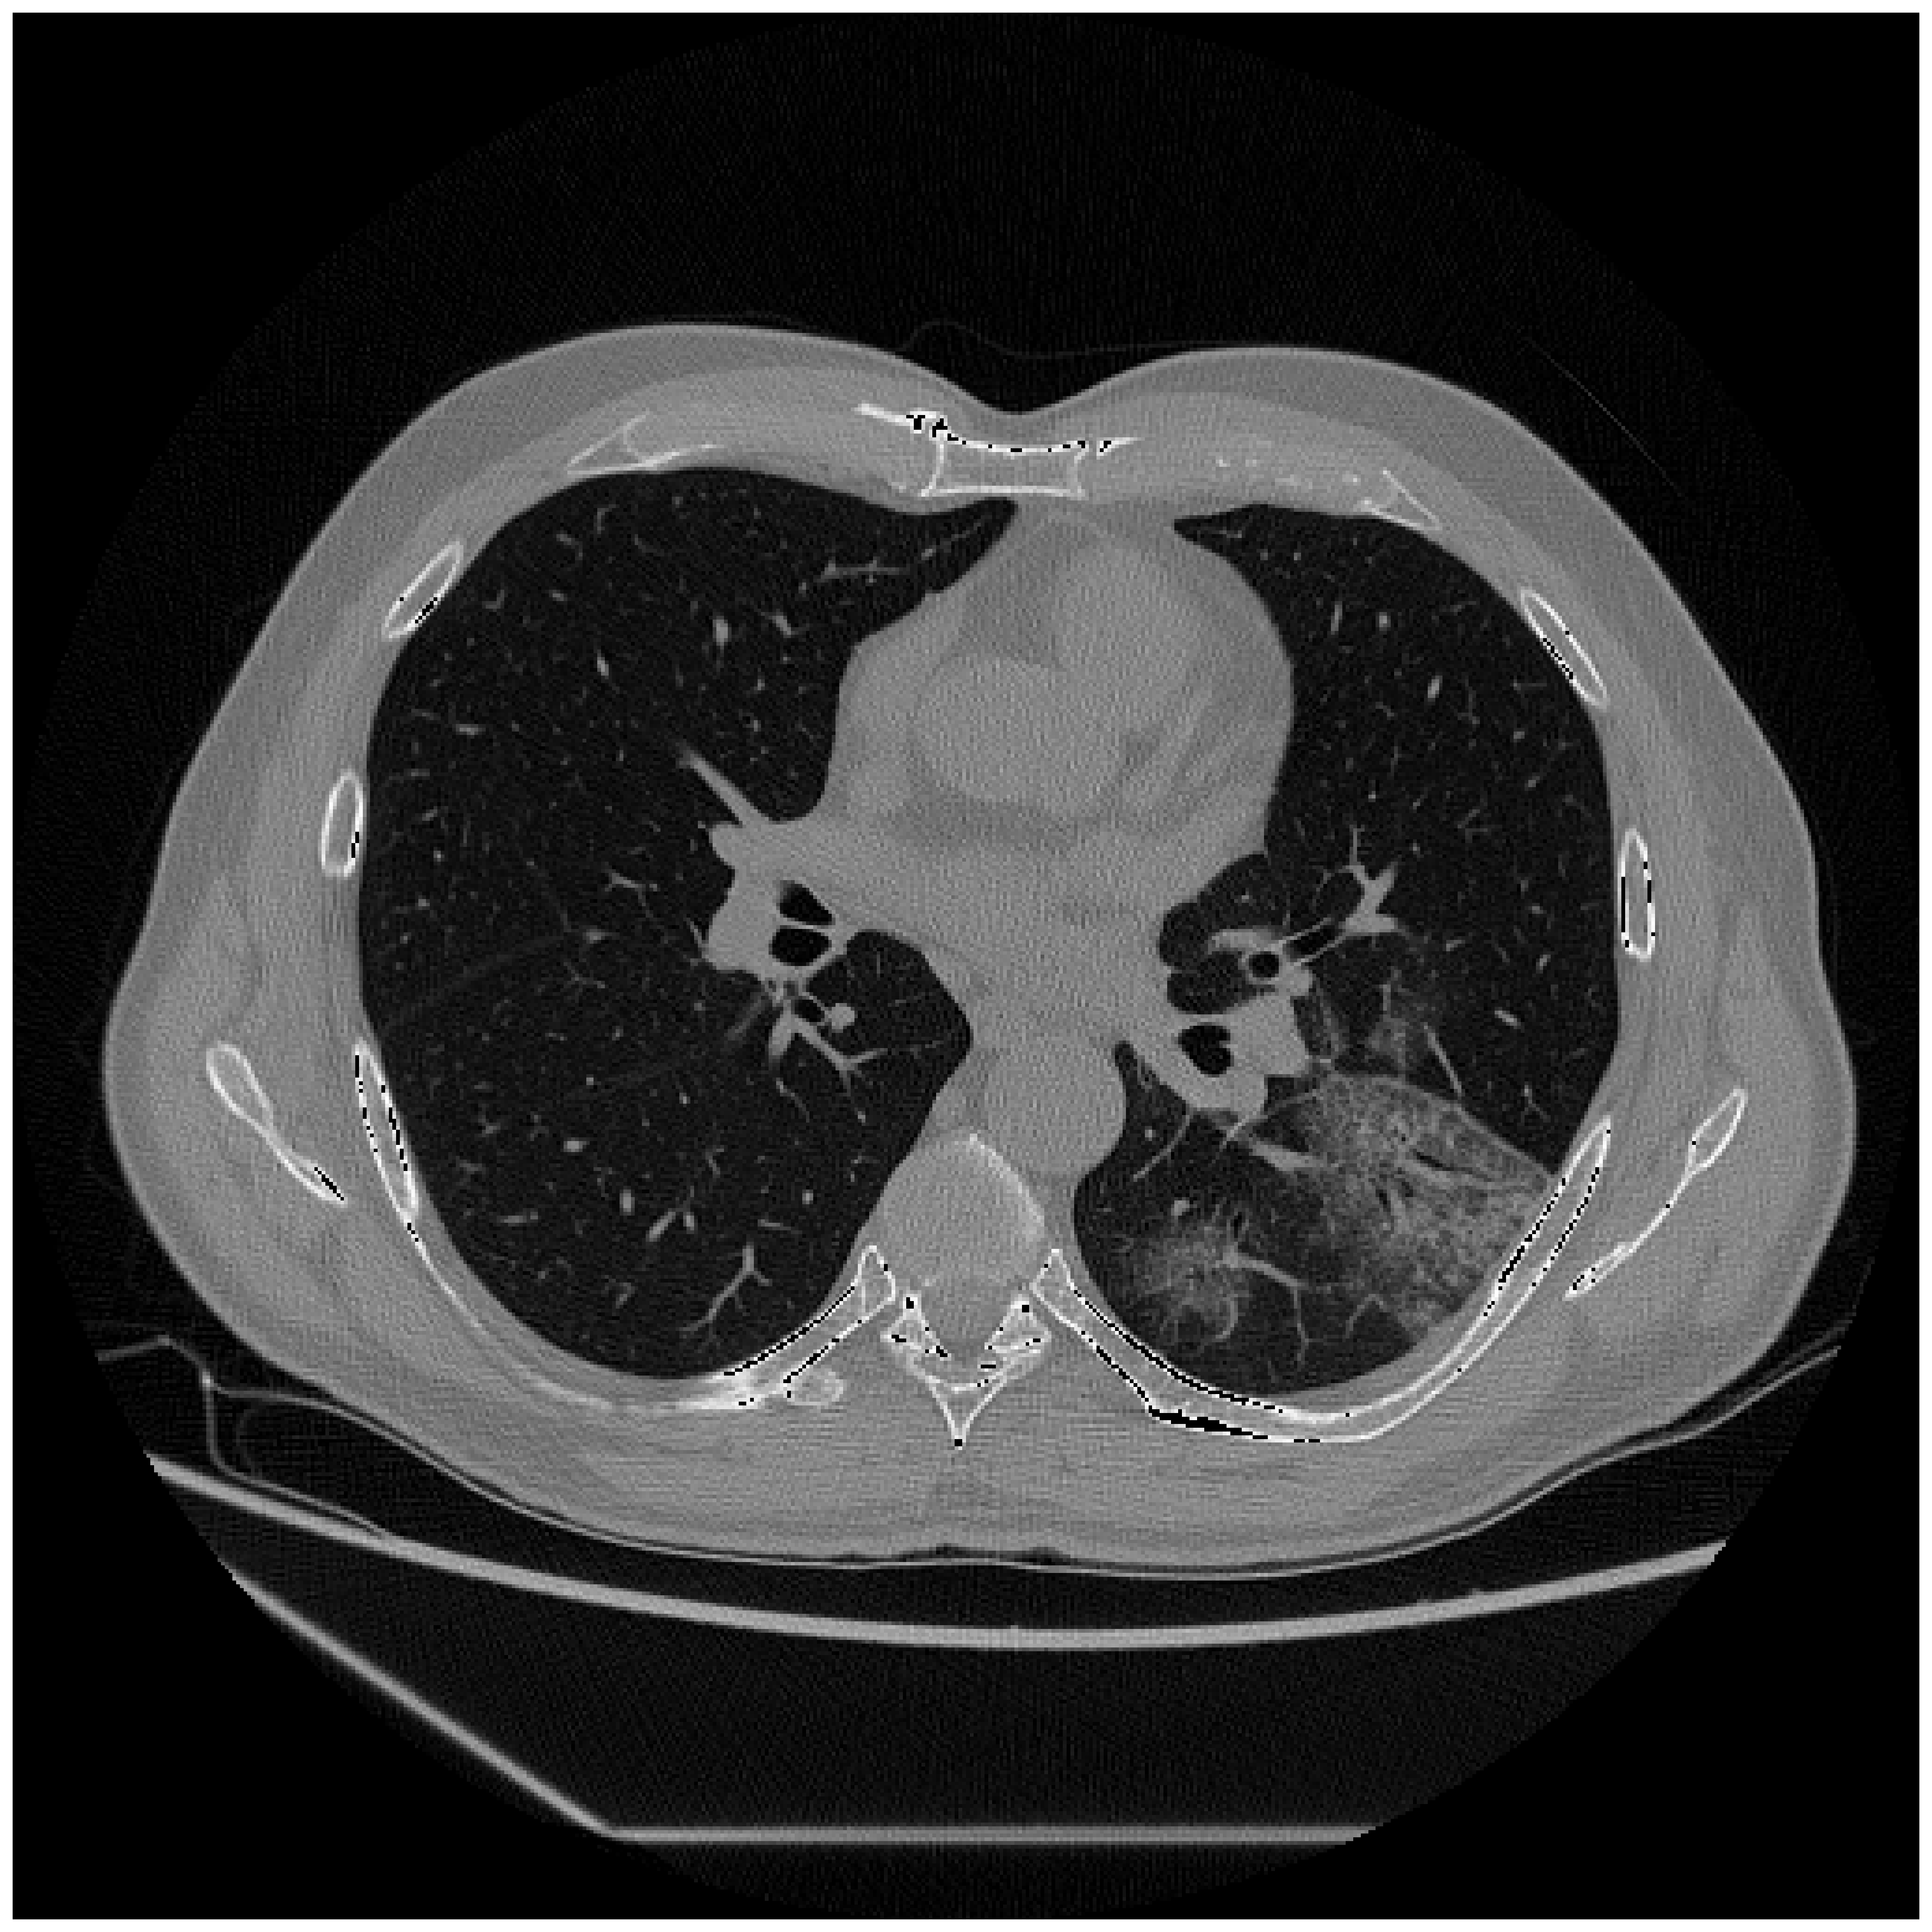
\includegraphics[scale=.12]{./img/GGO.png}			
		\end{column}
		\begin{column}{0.5\textwidth}
					\begin{block}{COVID-19}
					\begin{itemize}
						
						\item Viral(SARS-CoV-2) 
						
						\item Acute infectious disease
						
						\item Peculiar GGO and CS patterns
						
					\end{itemize}
				\end{block}			
				\begin{block}{Why Identify Them?}
					\begin{itemize}
						
						\item \textbf{To Help} diagnosis
						
						\item \textbf{To Monitor}:  
						\begin{itemize}
							\item the course of the disease
							
							\item the recovery of healed patients
						\end{itemize} 		
					\end{itemize}
				\end{block}				
		\end{column}
	\end{columns}	
	\end{frame}
\end{document} % What are GGO and why identiphy them?

\documentclass{standalone}
\begin{document}
	\setbeamertemplate{itemize/enumerate body begin}{\scriptsize}
	\setbeamertemplate{itemize/enumerate subbody begin}{\scriptsize}	
	%block settings	
	\setbeamercolor{block title}{fg=white, bg=mediumslateblue}
	\setbeamercolor{block body}{fg=black, bg=white}
	%alert block settings
	\setbeamercolor{block title alerted}{fg=white, bg=lightcarminepink}
	\setbeamercolor{block body alerted}{fg=black, bg=white}
	% example block settings
	\setbeamercolor{block title example}{fg=white, bg=mediumseagreen}
	\setbeamercolor{block body example}{fg=black, bg=white}
	
	\begin{frame}{State of the Art}{Current Methods, Problems and Solution}
		
		\begin{alertblock}{Current Segmentation Methods}
			Manual or Semi-automatic: 
			\begin{itemize}
				\item Time Consuming
				\item Requires Trained Personnel
				\item Subjected to Operator Expertise
			\end{itemize}
		\end{alertblock}
		
		\begin{block}{Characteristics of the Pipeline Implemented}
			\begin{itemize}
				\item Fully Automated: \emph{remove subjectivity and dependency of external operator}
				\item Fast: \emph{obtain results in a small amount of time }
			\end{itemize}
		\end{block}
	
		\begin{exampleblock}{Dataset}
			\begin{itemize}
				\item $83$ CT scans with annotation provided by \emph{Department of Experimental, Diagnostic and Specialty Medicine}
				\item $2$ Public Dataset
			\end{itemize}
		\end{exampleblock}
	\end{frame}
\end{document}% Why my work is important?

\documentclass{standalone}
\begin{document}
	\begin{frame}{Basic Idea}{Colour Quantization for Medical Image Segmentation}
		
		\begin{columns}
			\begin{column}{.4\textwidth}
				\begin{block}{GGO areas on CT Images}
					\begin{itemize}
						\item Similar Gray Level
						\item Spatially Displaced
					\end{itemize}				
				\end{block}
				\begin{block}{Basic Idea}
					\begin{itemize}
						\item \textbf{Colour Quantization}: Group Pixel Based on colour similarity
						\item \textbf{Colour Space}: Constructed by taking into accounts different information
					\end{itemize}
				\end{block}				
			\end{column}
			\begin{column}{.5\textwidth}
				\centering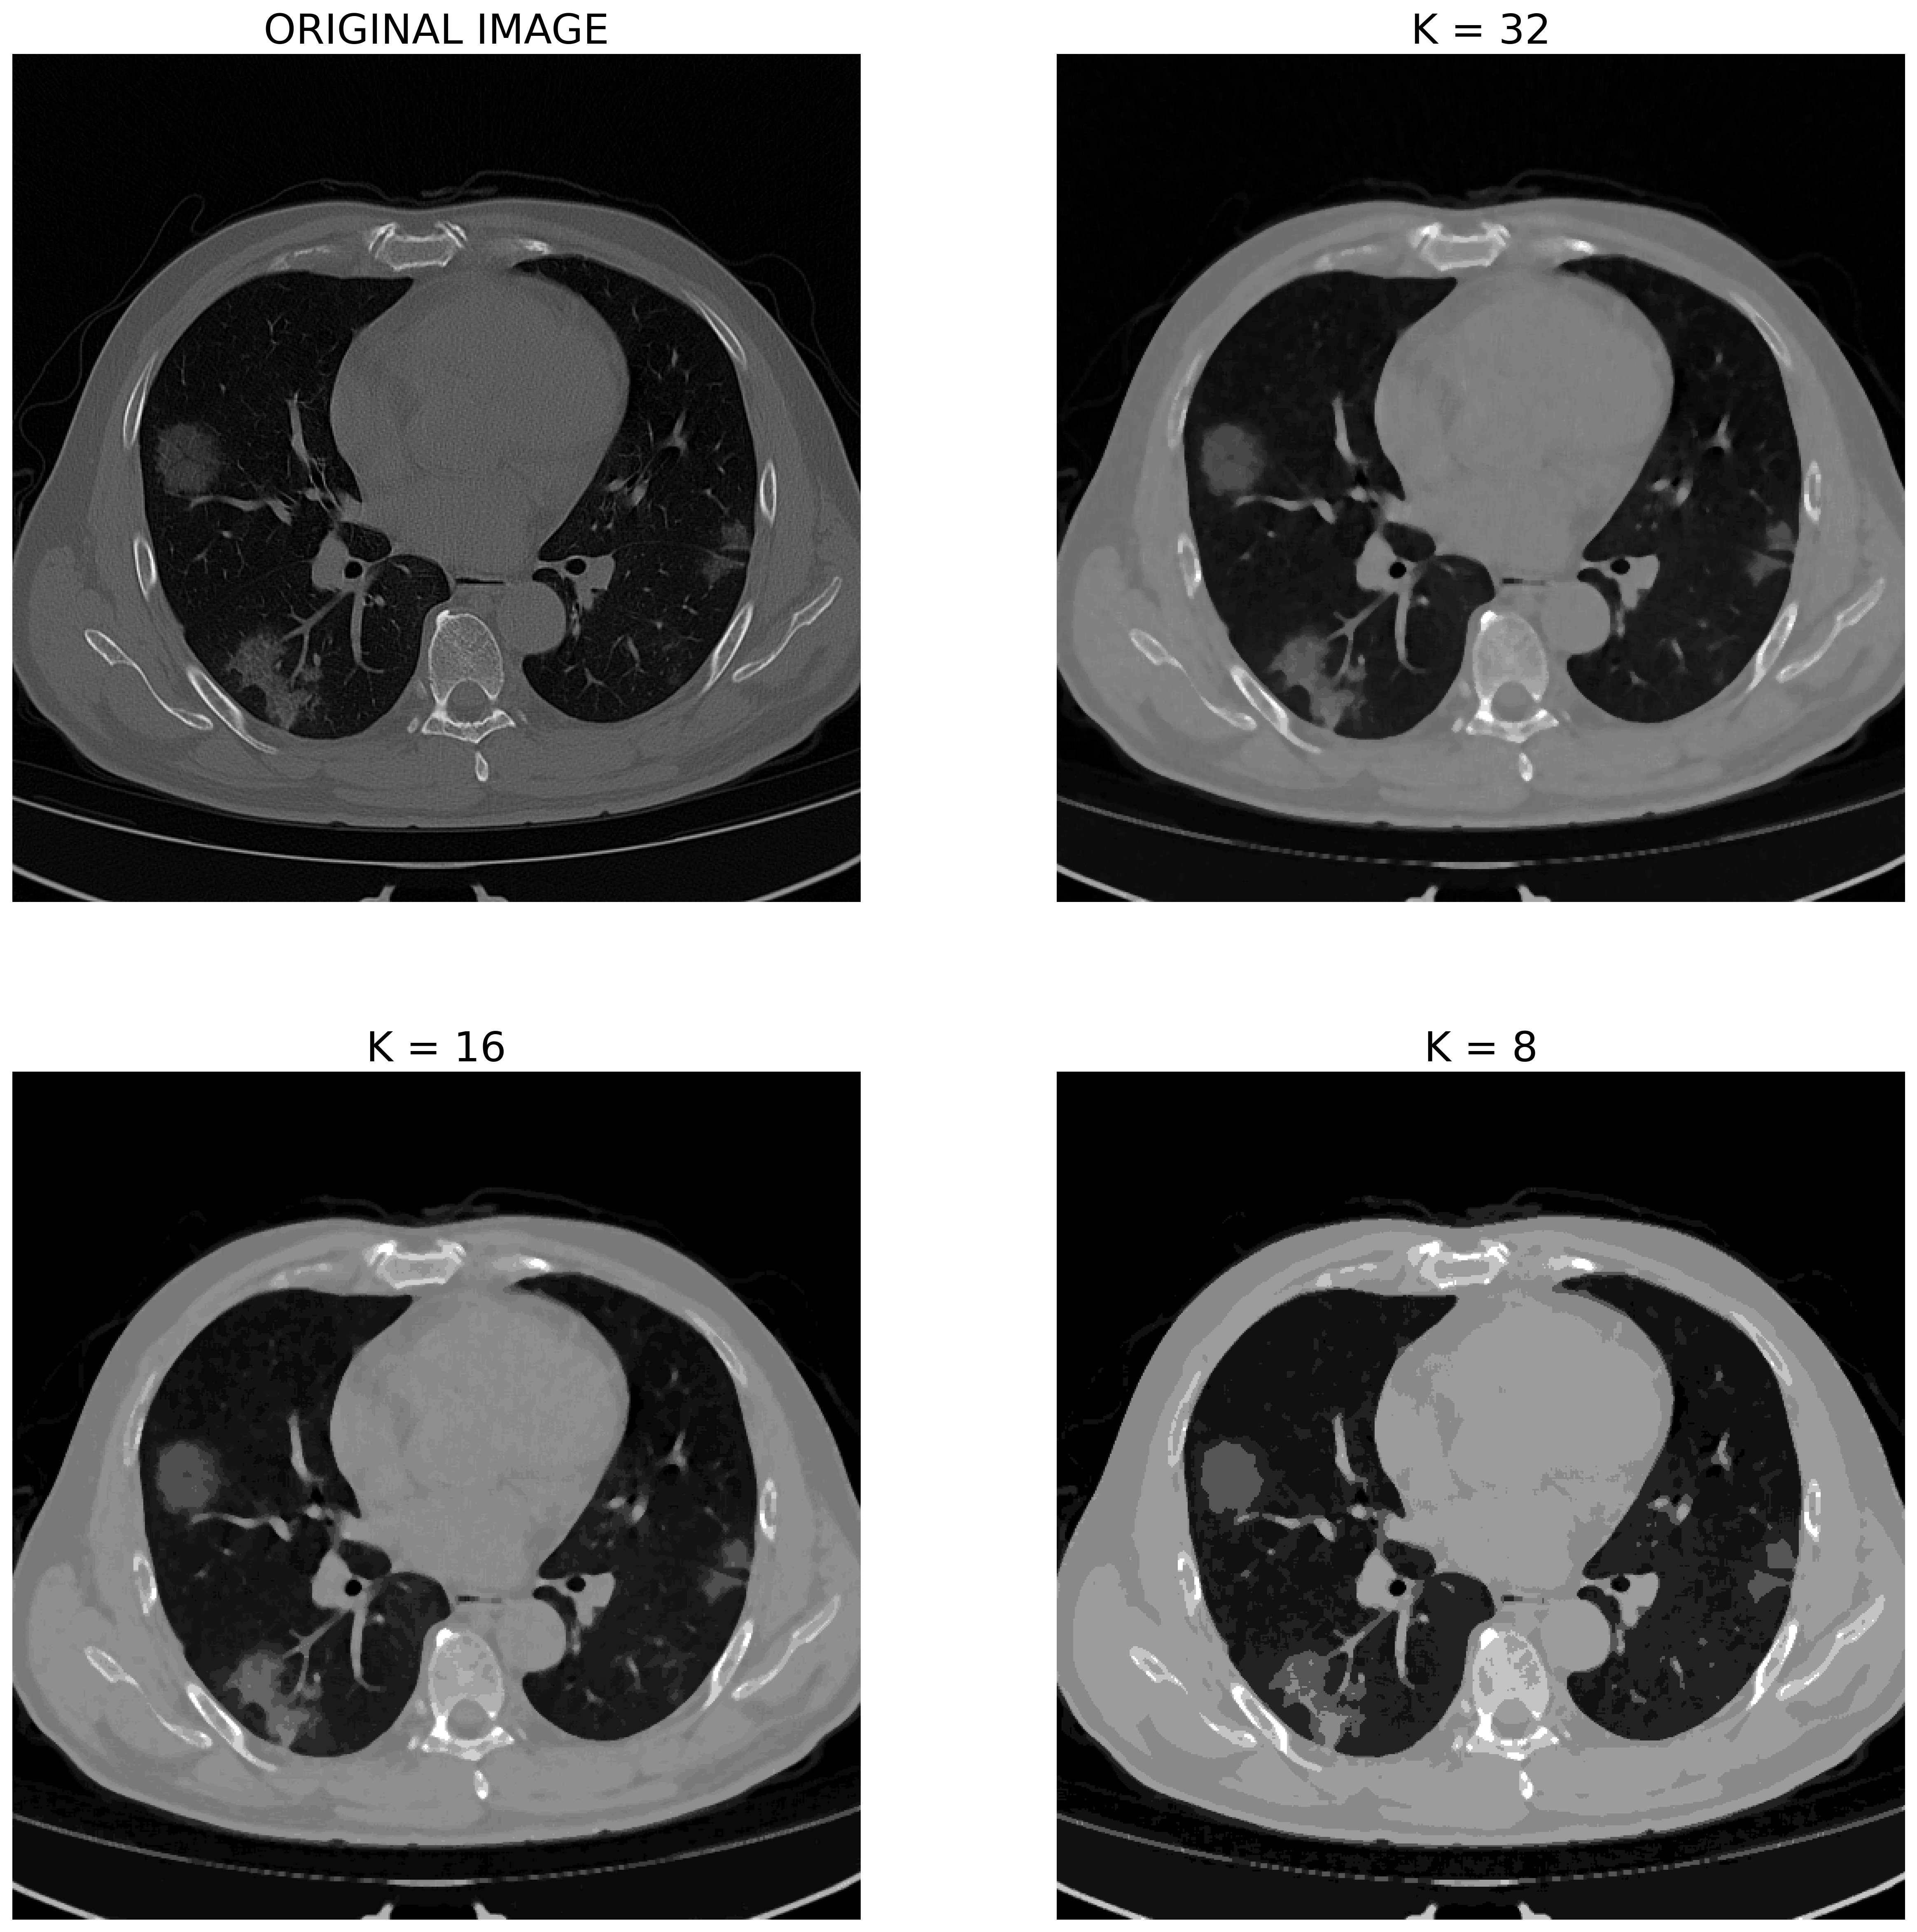
\includegraphics[width=\linewidth]{./img/ColorQuantization}
			\end{column}
		\end{columns}
	\end{frame}
\end{document} %Colour Quantization for Image Segmentation

\documentclass{standalone}
\begin{document}
	\setbeamertemplate{itemize/enumerate body begin}{\scriptsize}
	\setbeamertemplate{itemize/enumerate subbody begin}{\scriptsize}
	\begin{frame}{Implementation}{}		
		%\centering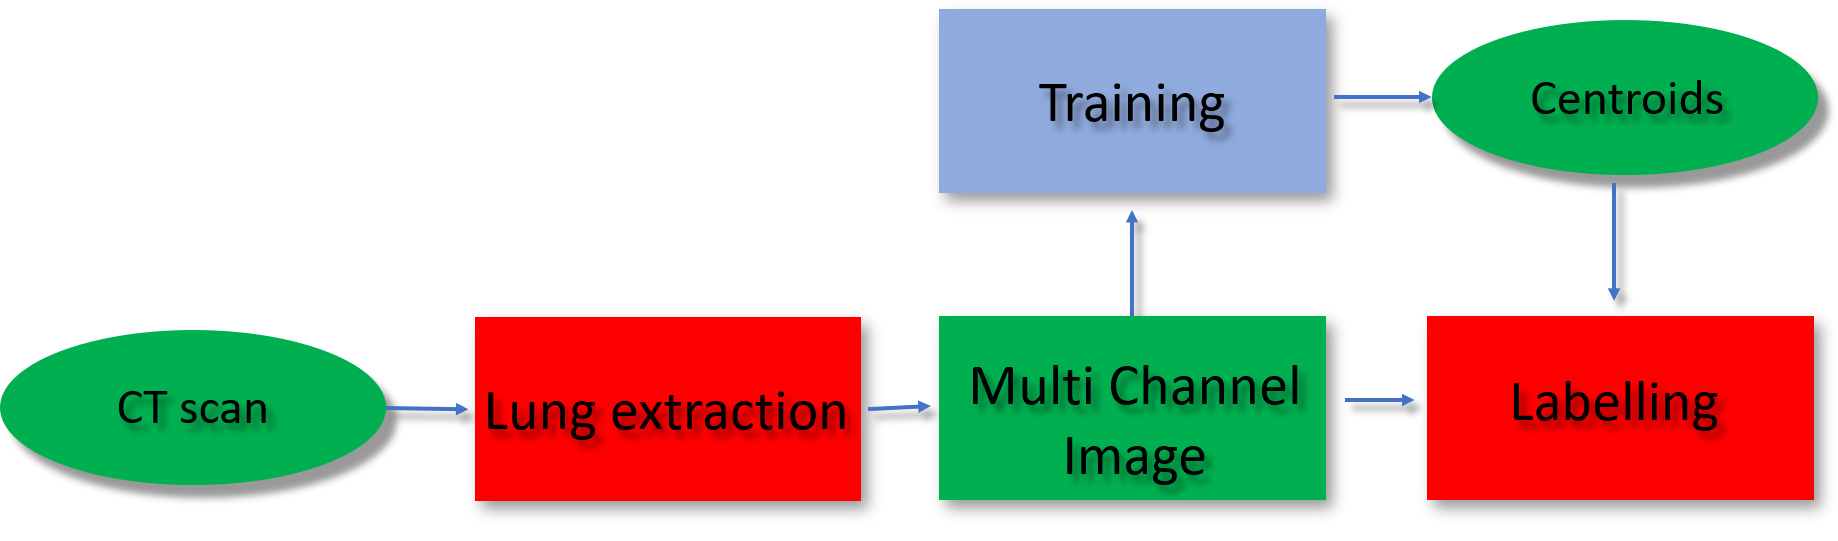
\includegraphics[width=\linewidth]{./img/Pipeline2}
		\begin{columns}
			\begin{column}{.4\textwidth}
				\centering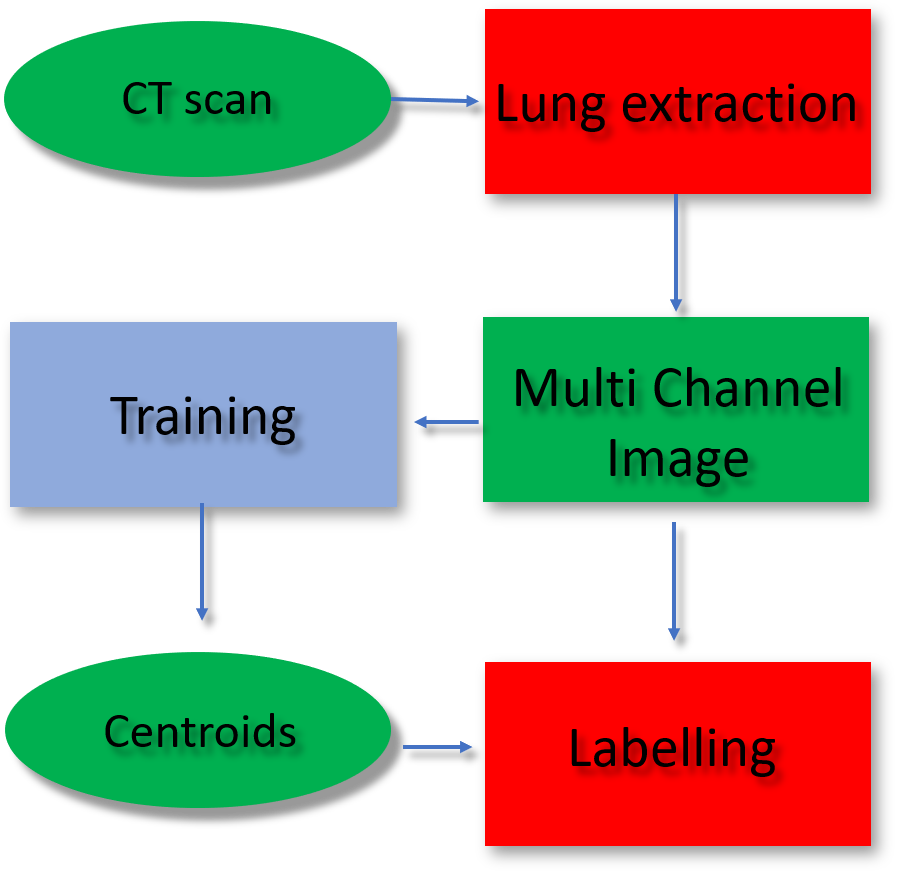
\includegraphics[width=\linewidth]{./img/Pipeline3}
			\end{column}
			\begin{column}{.4\textwidth}
				\begin{block}{}
					\begin{itemize}
						\item \textbf{LANGUAGE:} \textsf{Python} 
\includegraphics[width=.05\textwidth]{./img/python}
						\item \textbf{INSTALLATION:} \textsf{Setup}
						\item \textbf{OS:} Linux 
\includegraphics[width=.05\textwidth]{./img/linux} \&
					Windows 
\includegraphics[width=.05\textwidth]{./img/windows}
						\item \textbf{DOCUMENTATION:} Generated with Sphinx 
\includegraphics[width=.05\textwidth]{./img/sphinx}
						\item \textbf{CI:} Travis 
\includegraphics[width=.05\textwidth]{./img/travis} \& Appveyor 
\includegraphics[width=.05\textwidth]{./img/appveyor}
						\item \textbf{URL:} \url{https://github.com/RiccardoBiondi/segmentation} 
\includegraphics[width=.05\textwidth]{./img/github}
						\item \textbf{DEPENDENCIES:} \textsf{OpenCV} 
\includegraphics[width=.05\textwidth]{./img/OpenCV} \&
						\textsf{SimpleITK} 
\includegraphics[width=.05\textwidth]{./img/simpleitk} \&
						\textsf{Numpy} \includegraphics[width=.05\textwidth]{./img/numpy}
					\end{itemize}
				\end{block}
			\end{column}
		\end{columns}
	\end{frame}
\end{document}% The Workflow of the pipeline

\documentclass{standalone}
\begin{document}

	\subsection{Lung Extraction}
	
	The lung extraction is the first step of the pipeline which aims to isolate the region of interest and to remove the non-lung regions on CT scan. 
	This purpose is achieved by the following steps : 
	
	\begin{enumerate}
		\item Pre-Processing
		
		\item De-Noising
		
		\item Global Treshold
		
		\item Reconstruction of wrongly removed lung regions
		
		\item Selection of the largest connected region
	\end{enumerate}

	
		
\end{document} %Lung Segmentation How and Why

\documentclass{standalone}
\begin{document}
	\setbeamertemplate{itemize/enumerate body begin}{\scriptsize}
	\setbeamertemplate{itemize/enumerate subbody begin}{\scriptsize}
	\begin{frame}{Multi Channel Image}
			\begin{columns}
			\begin{column}{.6\textwidth}
				\centering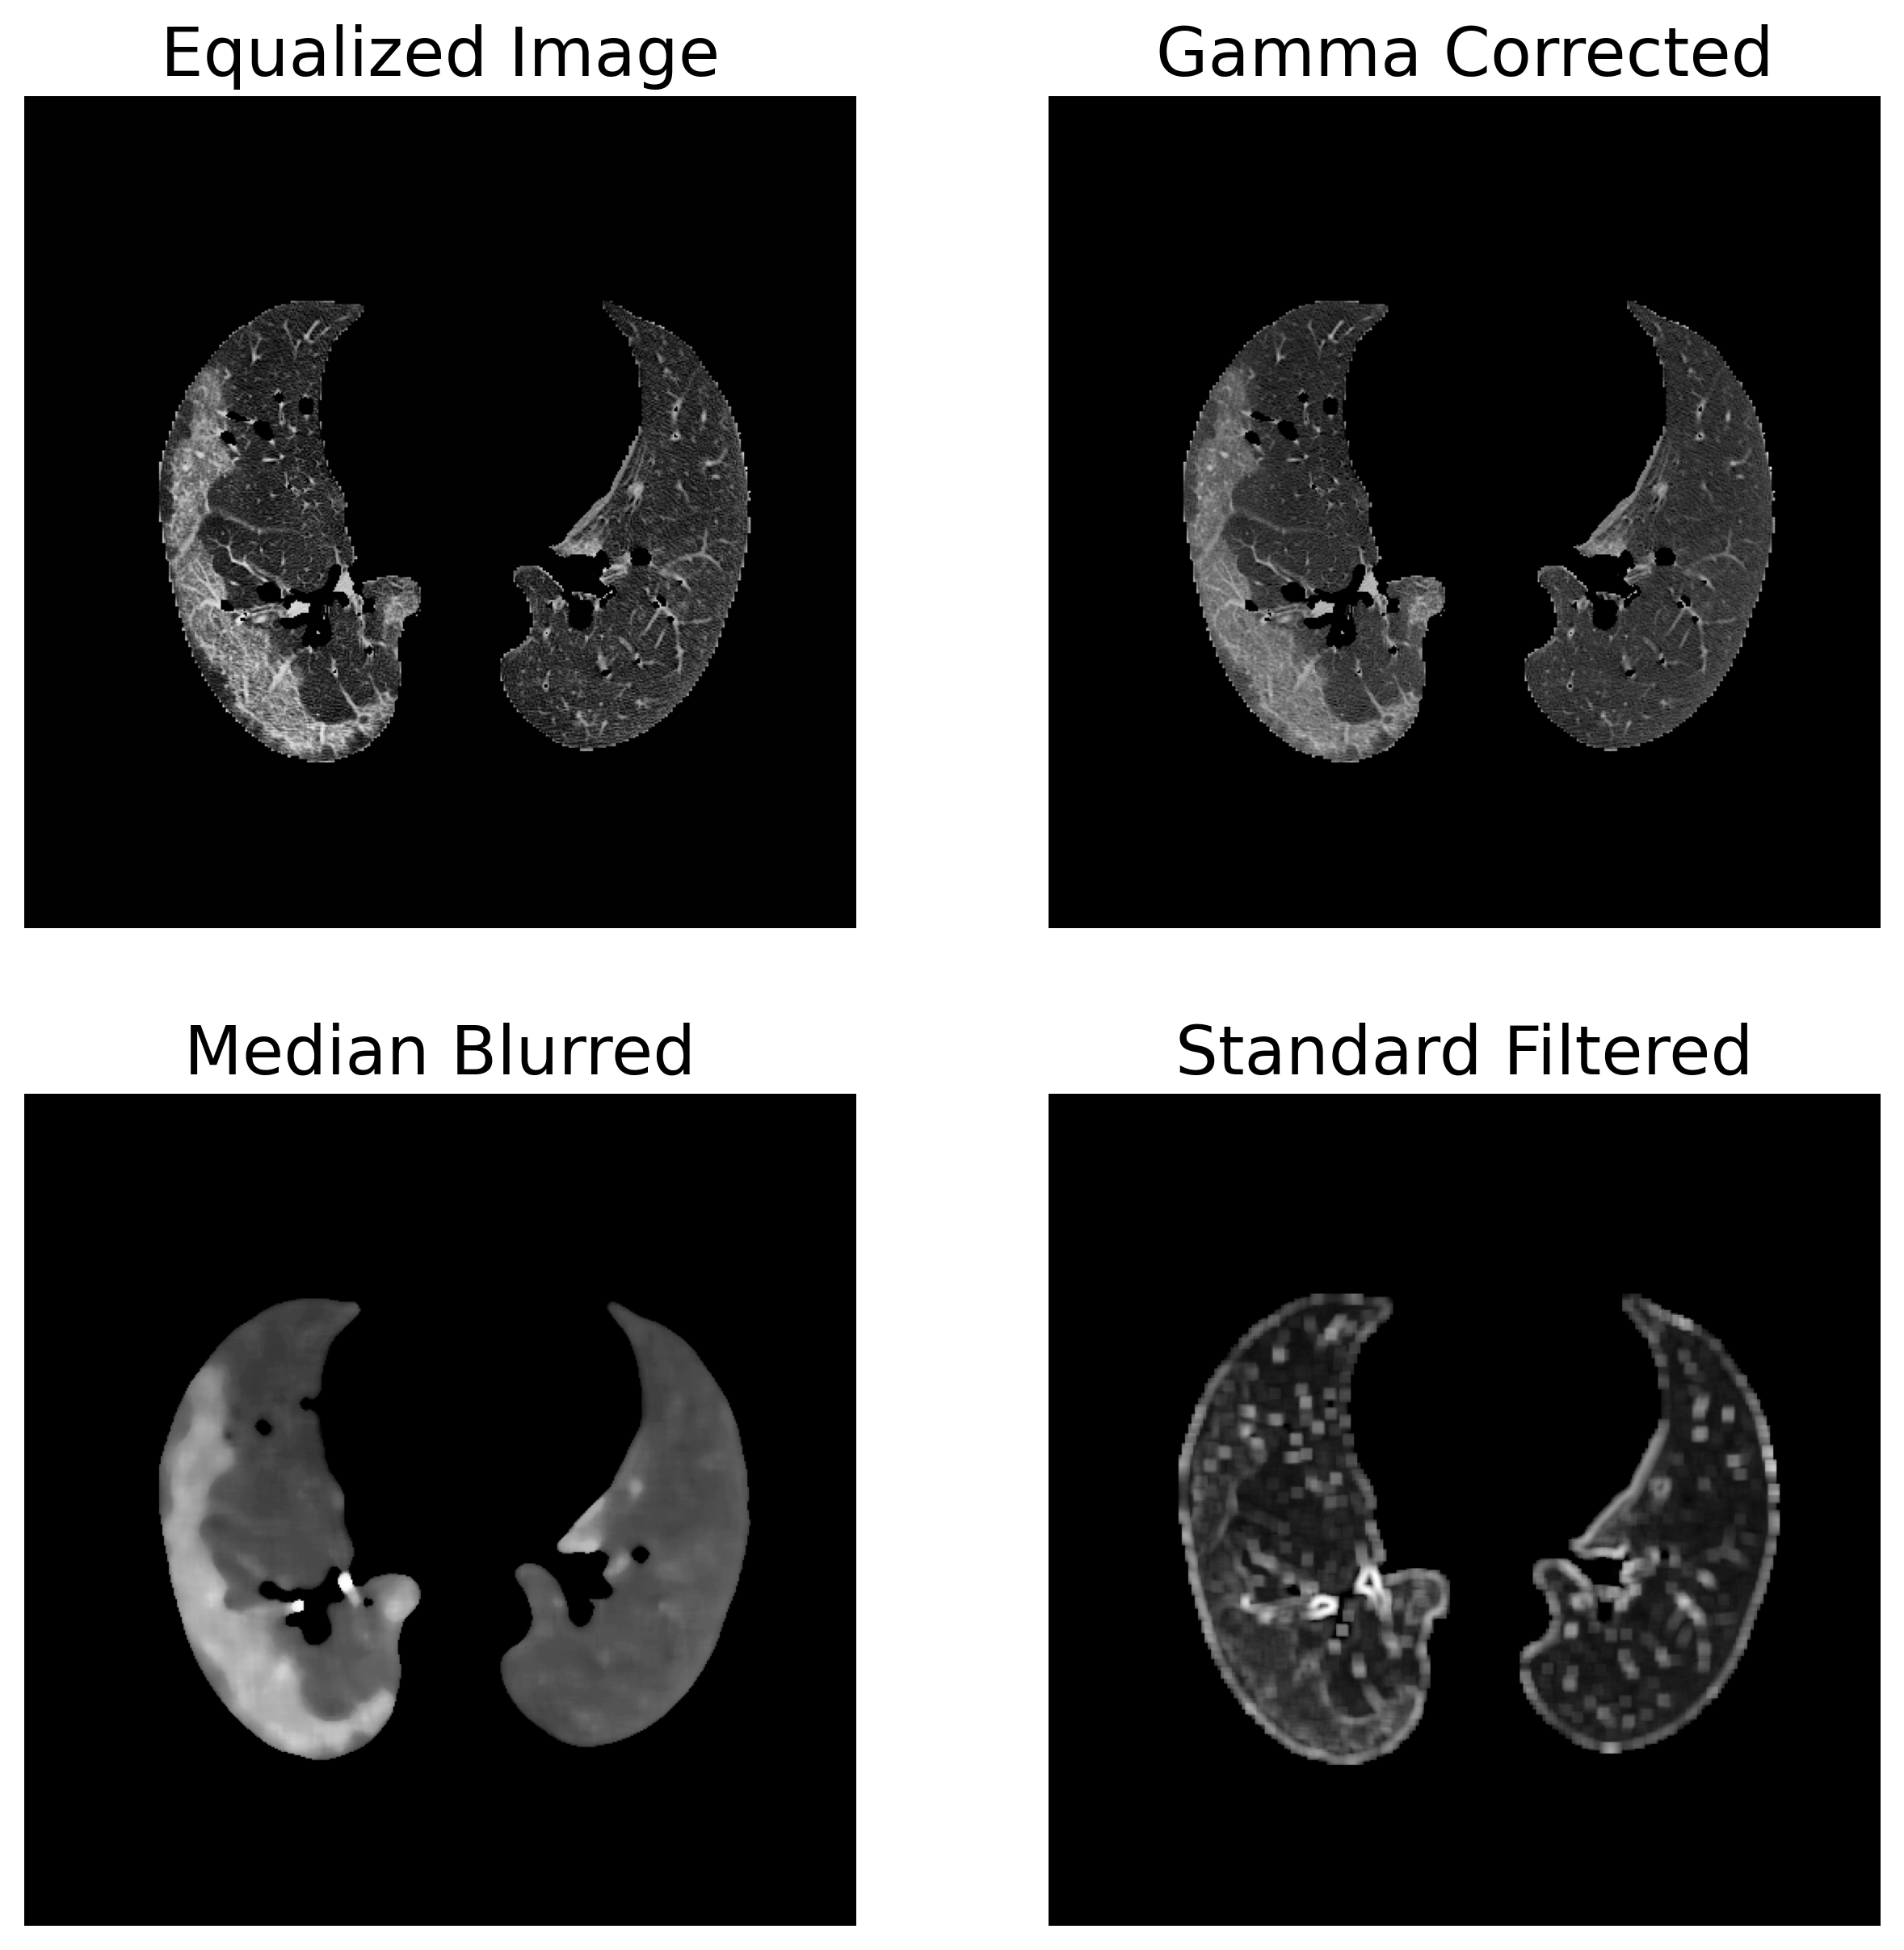
\includegraphics[scale=.33]{./img/Multi_Channel.png}
				\vspace{.2cm}			
			\end{column}
			\begin{column}{.3\textwidth}
				\begin{block}{Single Voxel}
					\begin{itemize}\setlength\itemsep{0.5em}
						\item Histogram Equalized 
						\item Gamma Corrected ($\gamma = 1.5$)
					\end{itemize}			
				\end{block}
%				\textbf{Single Voxel}:
%				\vspace{.3cm}
				\begin{block}{Neighbouring Voxels}
					\begin{itemize}\setlength\itemsep{0.5em}
						\item Median Blurred ($kernel\, size = 11$)
						\item Standard Deviation Map ($kernel\, size = 3$)						
					\end{itemize}
				\end{block}
				%\begin{itemize}\setlength\itemsep{0.5em}
					
				%	\item Histogram Equlization : 
						
					
				%	\item Gamma Corrected : 
						
					
			%	\end{itemize}			
				%\vspace{.5cm}
				%\textbf{Neighbouring Voxels}:
			%	\vspace{.3cm}
				%\begin{itemize}\setlength\itemsep{0.5em}
					
				%	\item Median Blurred
				%	
				%	\item Standard Deviation Map
				%	
				%\end{itemize}
			\end{column}		
		\end{columns}
		
	\end{frame}
\end{document} % how the multichannel image is build

\begin{document}
	
	\subsection{Training}
	
\end{document} % Centroid estimation

\documentclass{standalone}
\begin{document}
	\begin{frame}{Labelling}
		\begin{columns}
			\begin{column}{.4\textwidth}
				\centering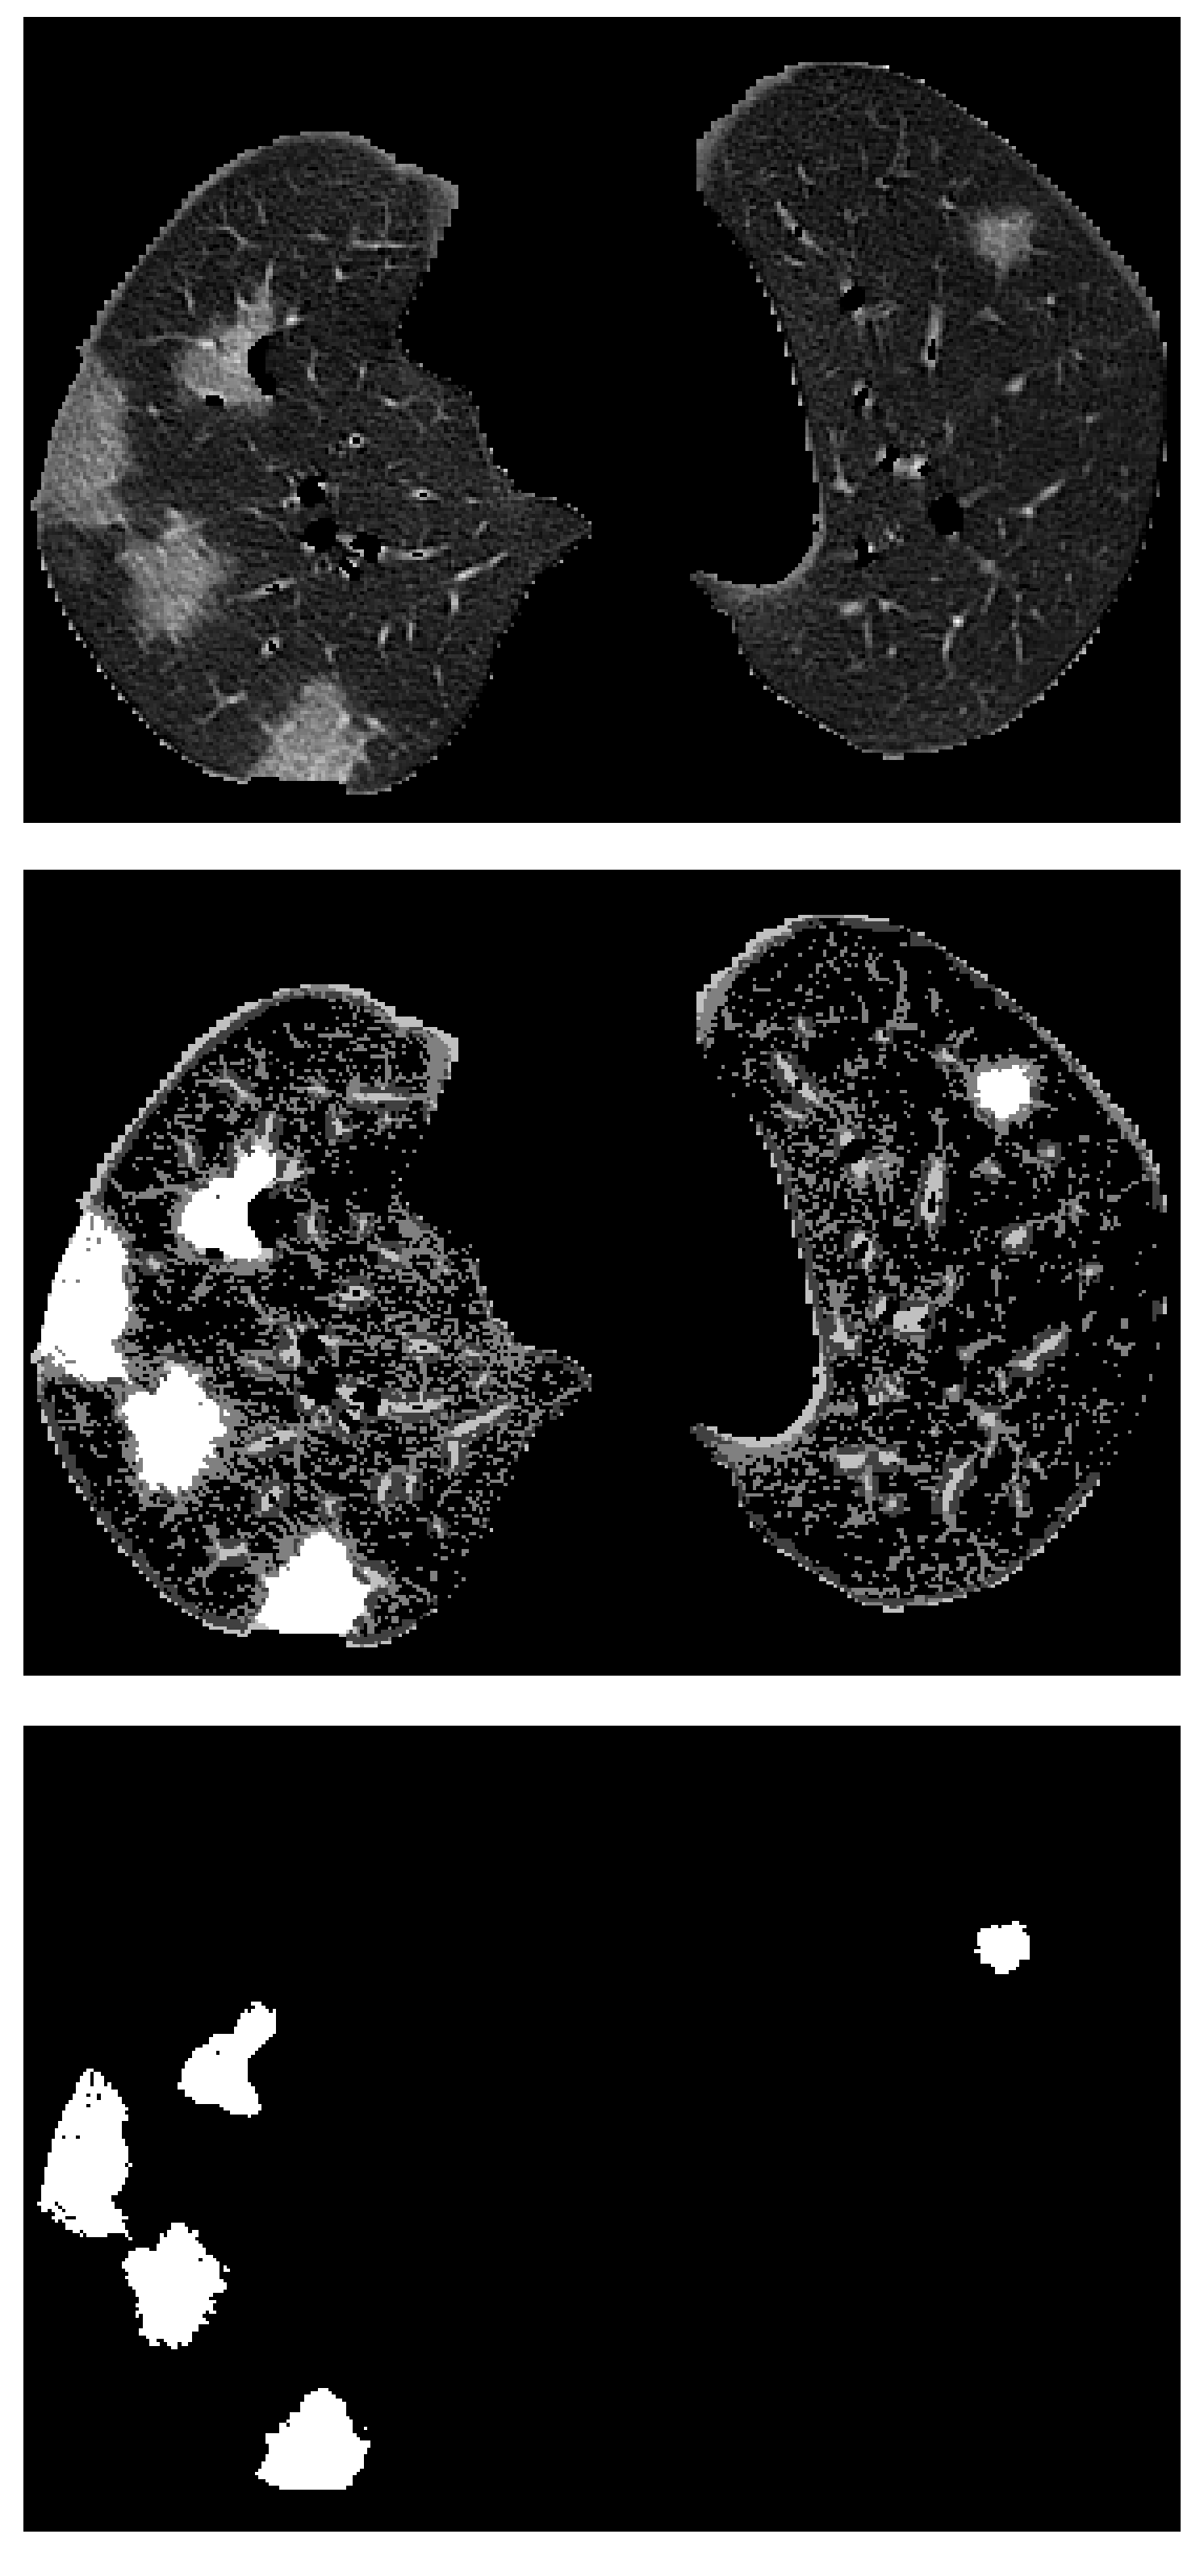
\includegraphics[width=.7\linewidth]{./img/labelling.png}
			\end{column}
		
			\begin{column}{.4\textwidth}
				
				\begin{block}{Input}
					\begin{itemize}
						\item Lung Extracted CT scan
						
						\item Centroids Set
					\end{itemize}
				\end{block}
				\begin{block}{}
					\begin{itemize}
						\item Build Multi Channel Image	
						
						\item Labelling by minimizing : 
						$\sum_{i=1}^{k}\sum_{S} \| x - \mu_i\|$		
						
						\item Select the labels corresponding to GGO as CS
						
						\item $45.65\pm 0.05\,ms$ per slice
						
						\item $DSC = 0.63 \pm 0.12$
								
					\end{itemize}
				\end{block}
			\end{column}
		\end{columns}
	\end{frame}
\end{document} % 

\documentclass{standalone}
\begin{document}
	\setbeamertemplate{itemize/enumerate body begin}{\scriptsize}
	\setbeamertemplate{itemize/enumerate subbody begin}{\scriptsize}
	\begin{frame}{Results}{Visual Comparison}

		%\begin{block}{}
		%	\centering\scriptsize{Comparison between the achieved results and manual annotation}
		%\end{block}

		\begin{columns}
			\begin{column}{.5\textwidth}
				\centering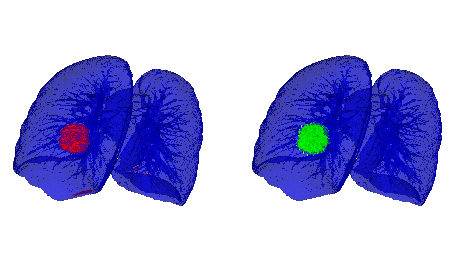
\includegraphics[width=\linewidth]{./img/3Dlesion}
			\end{column}
			\begin{column}{.4\textwidth}
				\begin{block}{}<1>
					\begin{itemize}
						\item \textcolor{green}{green}: semi-automated segmentation made by experts (some hours)
						\item \textcolor{red}{red}: automated pipeline results (less than \textit{3\,min})
					\end{itemize}
				\end{block}
			
			\end{column}
		\end{columns}
		\centering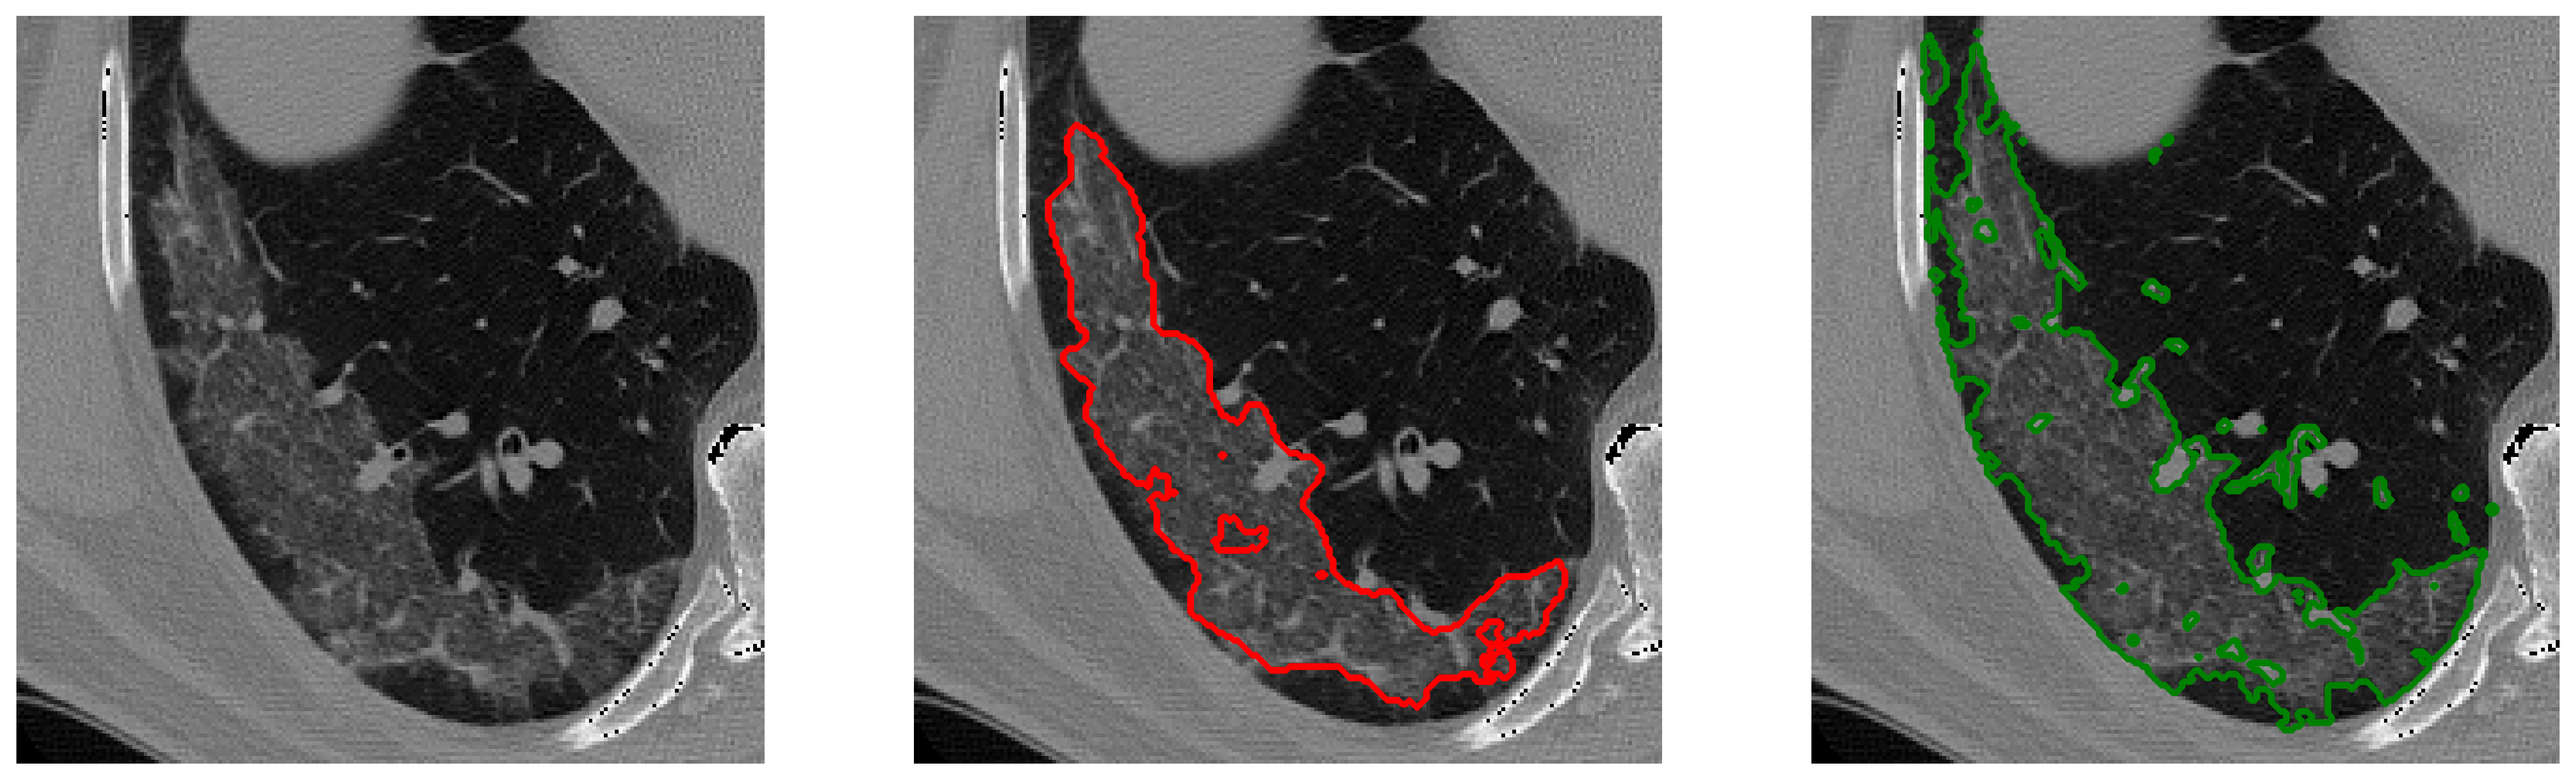
\includegraphics[width=\linewidth]{./img/zoom}
		\vspace{2mm}
	\end{frame}
\end{document} % visual comparison of the results

\documentclass{standalone}
\begin{document}
	%\begin{frame}{Results}{Expert Blind Evaluation}
	%	\begin{block}{}
	%		\centering\scriptsize{Blind evaluation by $3$ experts with at least $2$ years of experience}			
	%	\end{block}
	
	%	\centering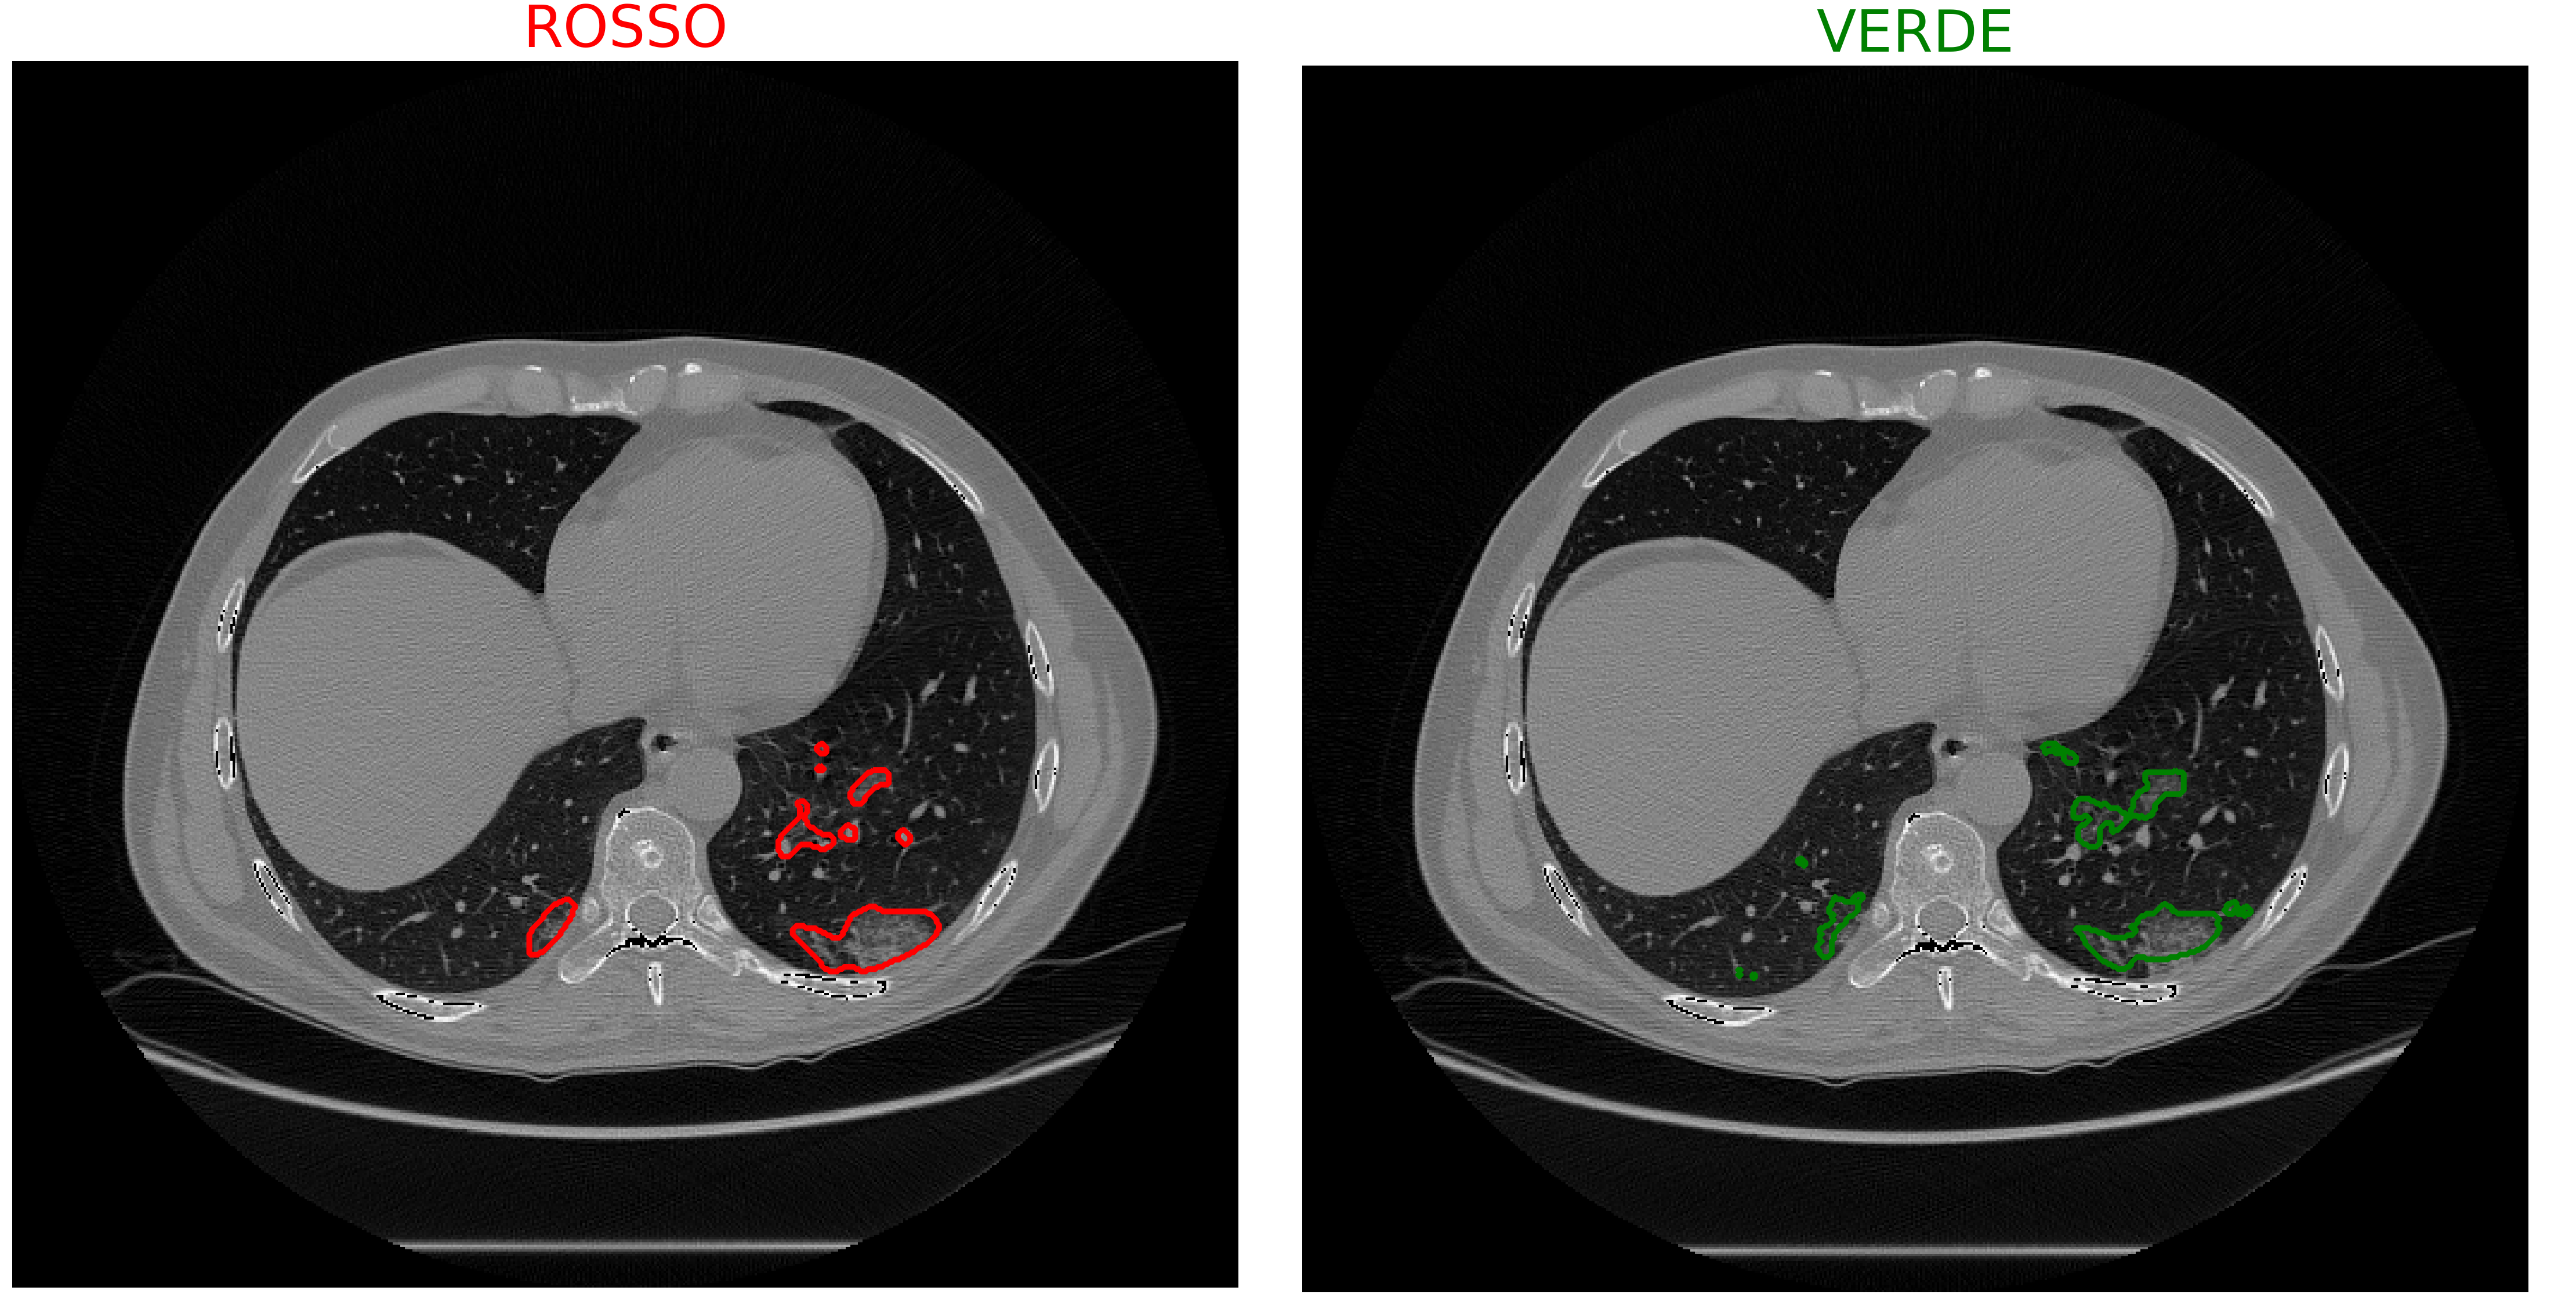
\includegraphics[width=.7\linewidth]{./img/BlindEval}
		
	%	\begin{block}{Blind Evaluation Results}
	%		\centering
	%		\begin{itemize}
	%			\item \scriptsize{Internal accordance less than $50\,\%$ in 4 of 7 cases}
	%			\item \scriptsize{Better Pipeline performance in 3 out of 7 cases}
	%		\end{itemize}
	%	\end{block}
	%\end{frame}
	\setbeamertemplate{itemize/enumerate body begin}{\scriptsize}
	\setbeamertemplate{itemize/enumerate subbody begin}{\scriptsize}
	\begin{frame}{Results}{Experts Blind Evaluation}
		%\begin{block}{}\scriptsize
		%	$7$ segmentations submitted to $3$ experts with at least $2$ years of experience
		%\end{block}
		\begin{block}{}
			\begin{itemize}
				\item $7$ segmentations submitted to $3$ experts (\emph{with at least $2$ years of experience})
				\item $3$ independent evaluations for each scans 
				\item Internal accordance lower than $50\%$
				
			\end{itemize}
		\end{block}
		\begin{columns}
			\begin{column}{.6\textwidth}
				\centering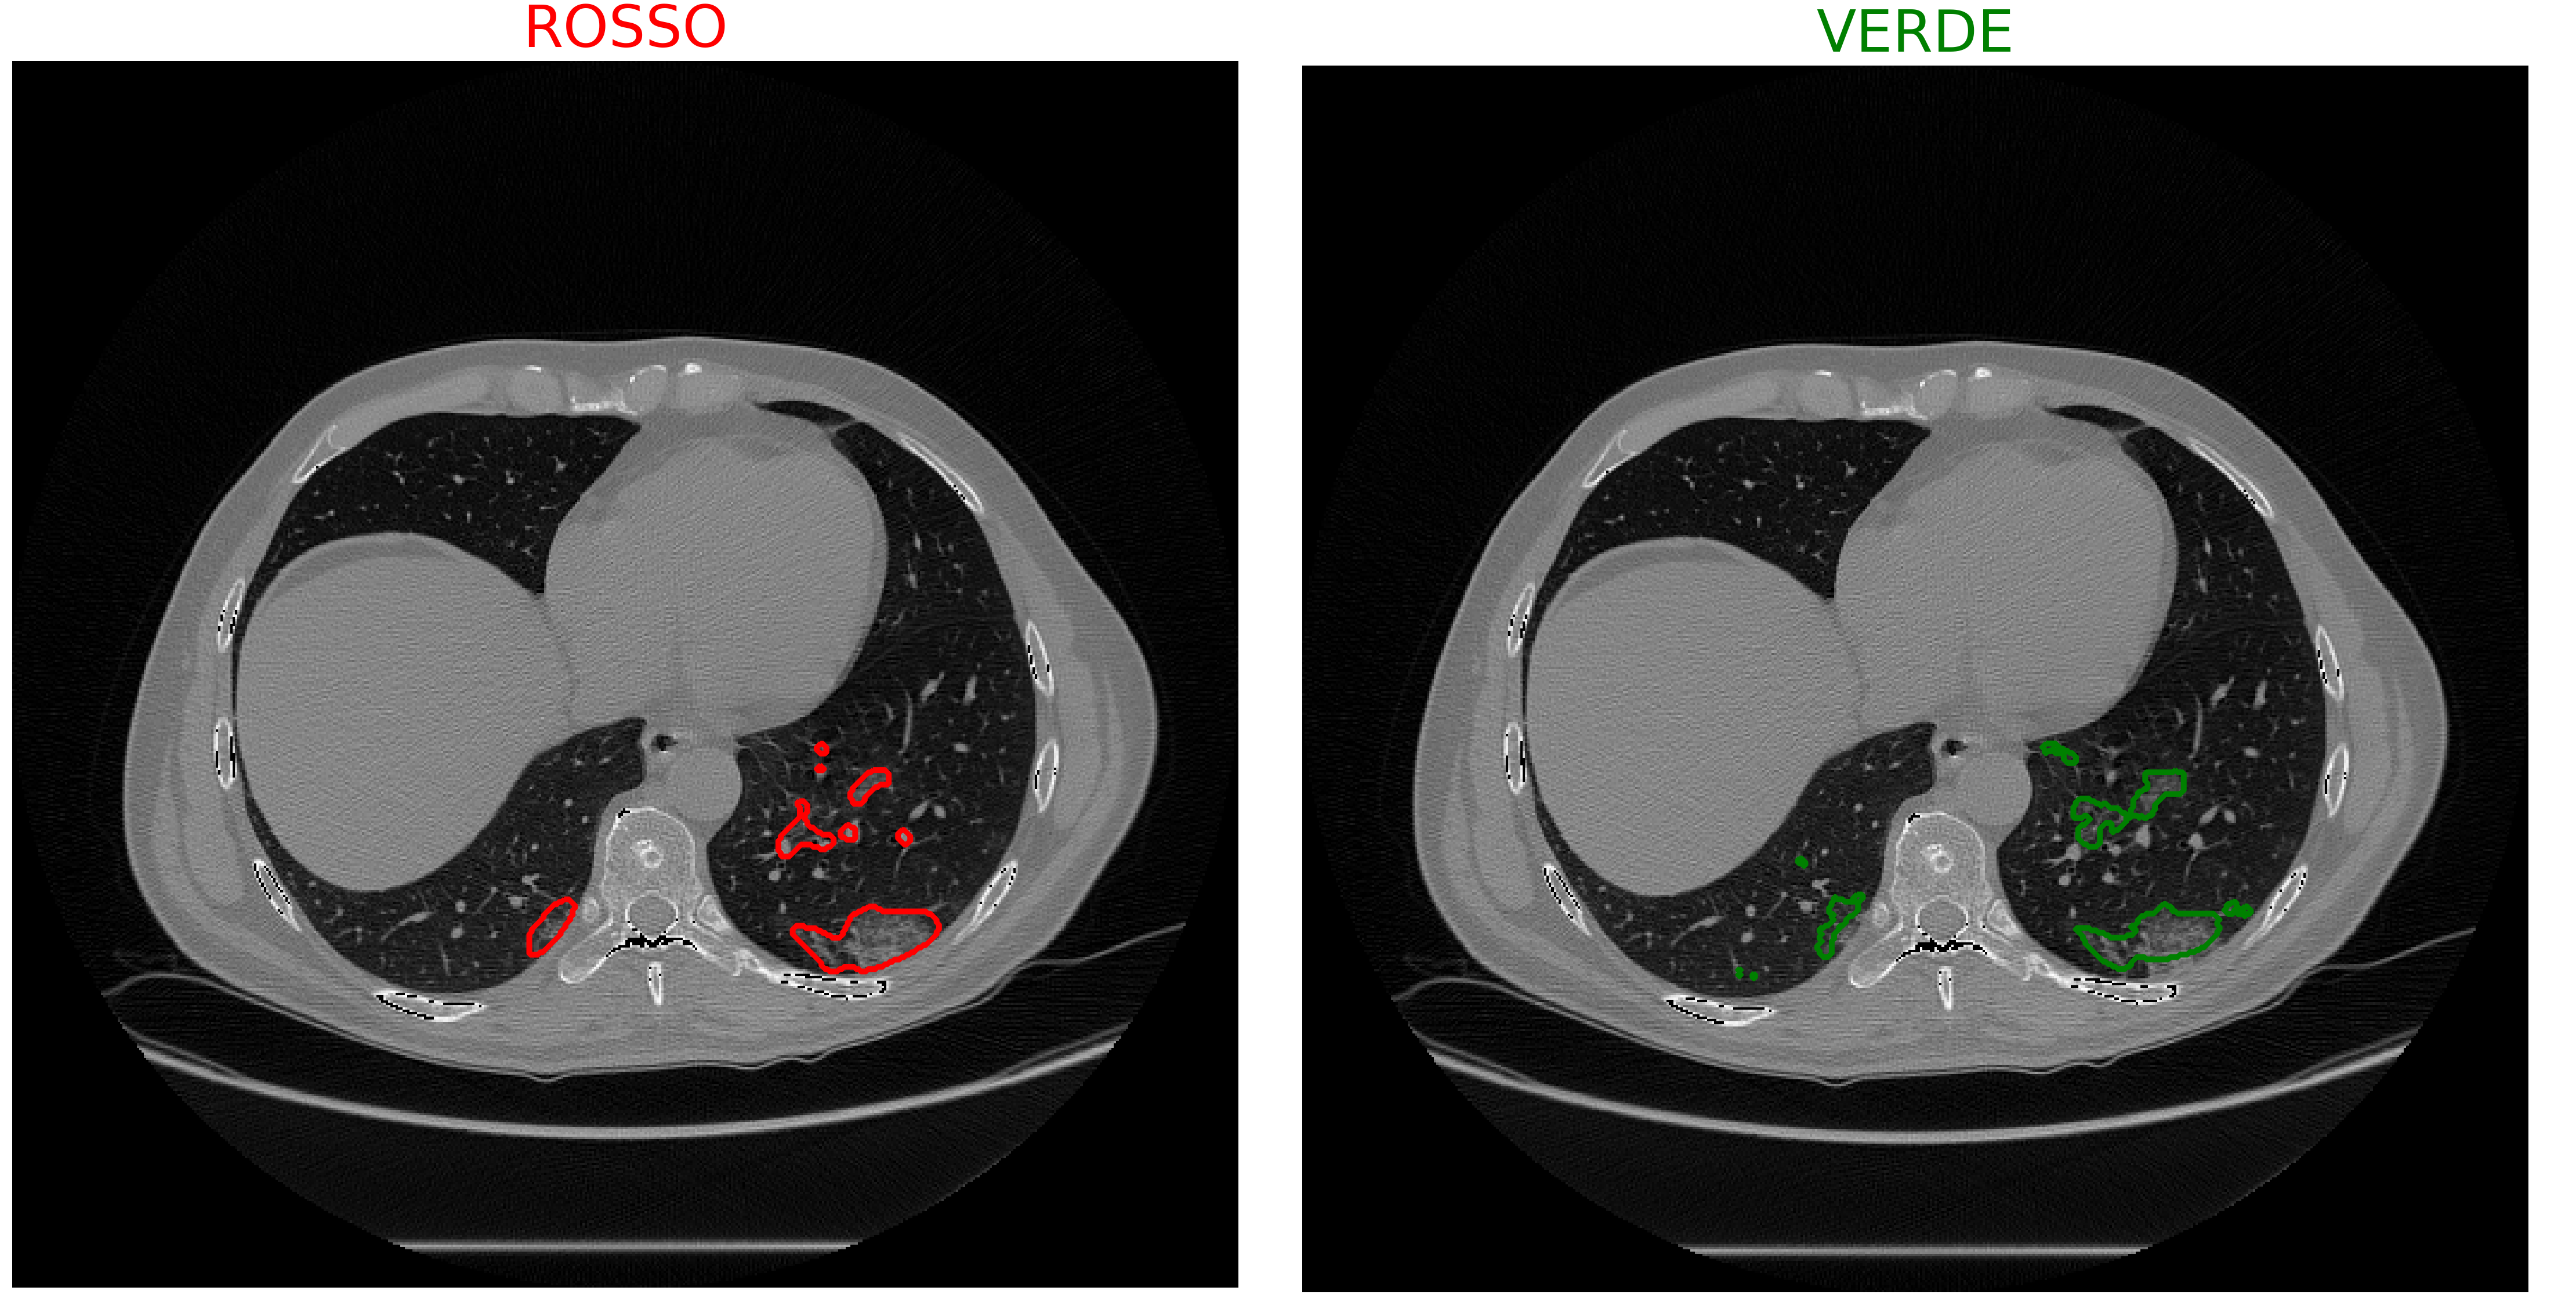
\includegraphics[width=\linewidth]{./img/BlindEval}
			\end{column}
			\begin{column}{.3\textwidth}
				\begin{block}{}\scriptsize
					Percentage of positive assessments
					\begin{table}
						\begin{tabular}{|l|l|}
							\hline
							pipeline 	& $32 \%$\\ \hline
							annotation 	& $33 \%$\\ \hline
							none 		& $35 \%$\\	\hline			
						\end{tabular}
					\end{table}
				\end{block}
			\end{column}
		\end{columns}
		%\begin{block}{}
		%	\begin{itemize}
		%		\item $3$ independent evaluations for each scans 
		%		\item Internal accordance lower than $50\%$
		%	\end{itemize}
		%\end{block}
	\end{frame}

\end{document}  % expert evaluation results

\documentclass{standalone}
\begin{document}
	\begin{frame}{Conclusion}{}
		\begin{block}{}
			
			\centering
			\begin{itemize}\setlength\itemsep{0.5em}
				\item \textbf{Achieved a segmentation in less than $3\,min$}
				\item \textbf{Fully automated}
				\item \textbf{Colour quantization has shown to be a suitable approach to face this kind of problems}
				\item \textbf{Interaction with specialised personnel needed to improve results}
			\end{itemize}
		\end{block}
	\end{frame}
\end{document}


% starting backup slice
\appendix
\setbeamertemplate{page number in head/foot}{} % no numbering

%\documentclass{standalone}
\begin{document}
	\setbeamertemplate{itemize/enumerate body begin}{\scriptsize}
	\setbeamertemplate{itemize/enumerate subbody begin}{\scriptsize}
	\begin{frame}{Implementation}
		\begin{block}{}
			\begin{columns}
				\begin{column}{.75\textwidth}
					\begin{itemize}
						\item \textbf{LANGUAGE:} \textsf{Python} 
\includegraphics[width=.03\textwidth]{./img/python}
						\item \textbf{INSTALLATION:} \textsf{Setup}
						\item \textbf{OS:} Linux 
\includegraphics[width=.03\textwidth]{./img/linux} \&
										   Windows 
\includegraphics[width=.03\textwidth]{./img/windows}
						\item \textbf{DOCUMENTATION:} fully documented by Sphinx 
\includegraphics[width=.04\textwidth]{./img/sphinx}
						\item \textbf{CI:} Travis 
\includegraphics[width=.03\textwidth]{./img/travis} \& Appveyor 
\includegraphics[width=.03\textwidth]{./img/appveyor}
						\item \textbf{URL:} \url{https://github.com/RiccardoBiondi/segmentation} 
\includegraphics[width=.03\textwidth]{./img/github}
						\item \textbf{DEPENDENCIES:} \textsf{OpenCV} 
\includegraphics[width=.03\textwidth]{./img/OpenCV} \&
								\textsf{SimpleITK} 
\includegraphics[width=.03\textwidth]{./img/simpleitk} \&
								\textsf{Numpy} \includegraphics[width=.03\textwidth]{./img/numpy}
					\end{itemize}
				\end{column}
			\end{columns}
		\end{block}
	\end{frame}
\end{document}


%\documentclass{standalone}
\begin{document}
	\begin{frame}[noframenumbering]{Future Development}
		\begin{block}{}
			\begin{columns}
				\begin{column}{.5\textwidth}
					\begin{itemize}
						\item Exploit of 3D structure
						\item Fine Training 
						\item Embedding of Spatial Information
						\item Improve Sensitivity
					\end{itemize}
				\end{column}
			\end{columns}			
		\end{block}
	\end{frame}
\end{document} % 

\documentclass{standalone}
\begin{document}
	\begin{frame}[noframenumbering]{Max Eigenvalues Map}{Bronchial Structure Removal}
		\begin{columns}[b]
		
			\begin{column}{.4\textwidth}
				\centering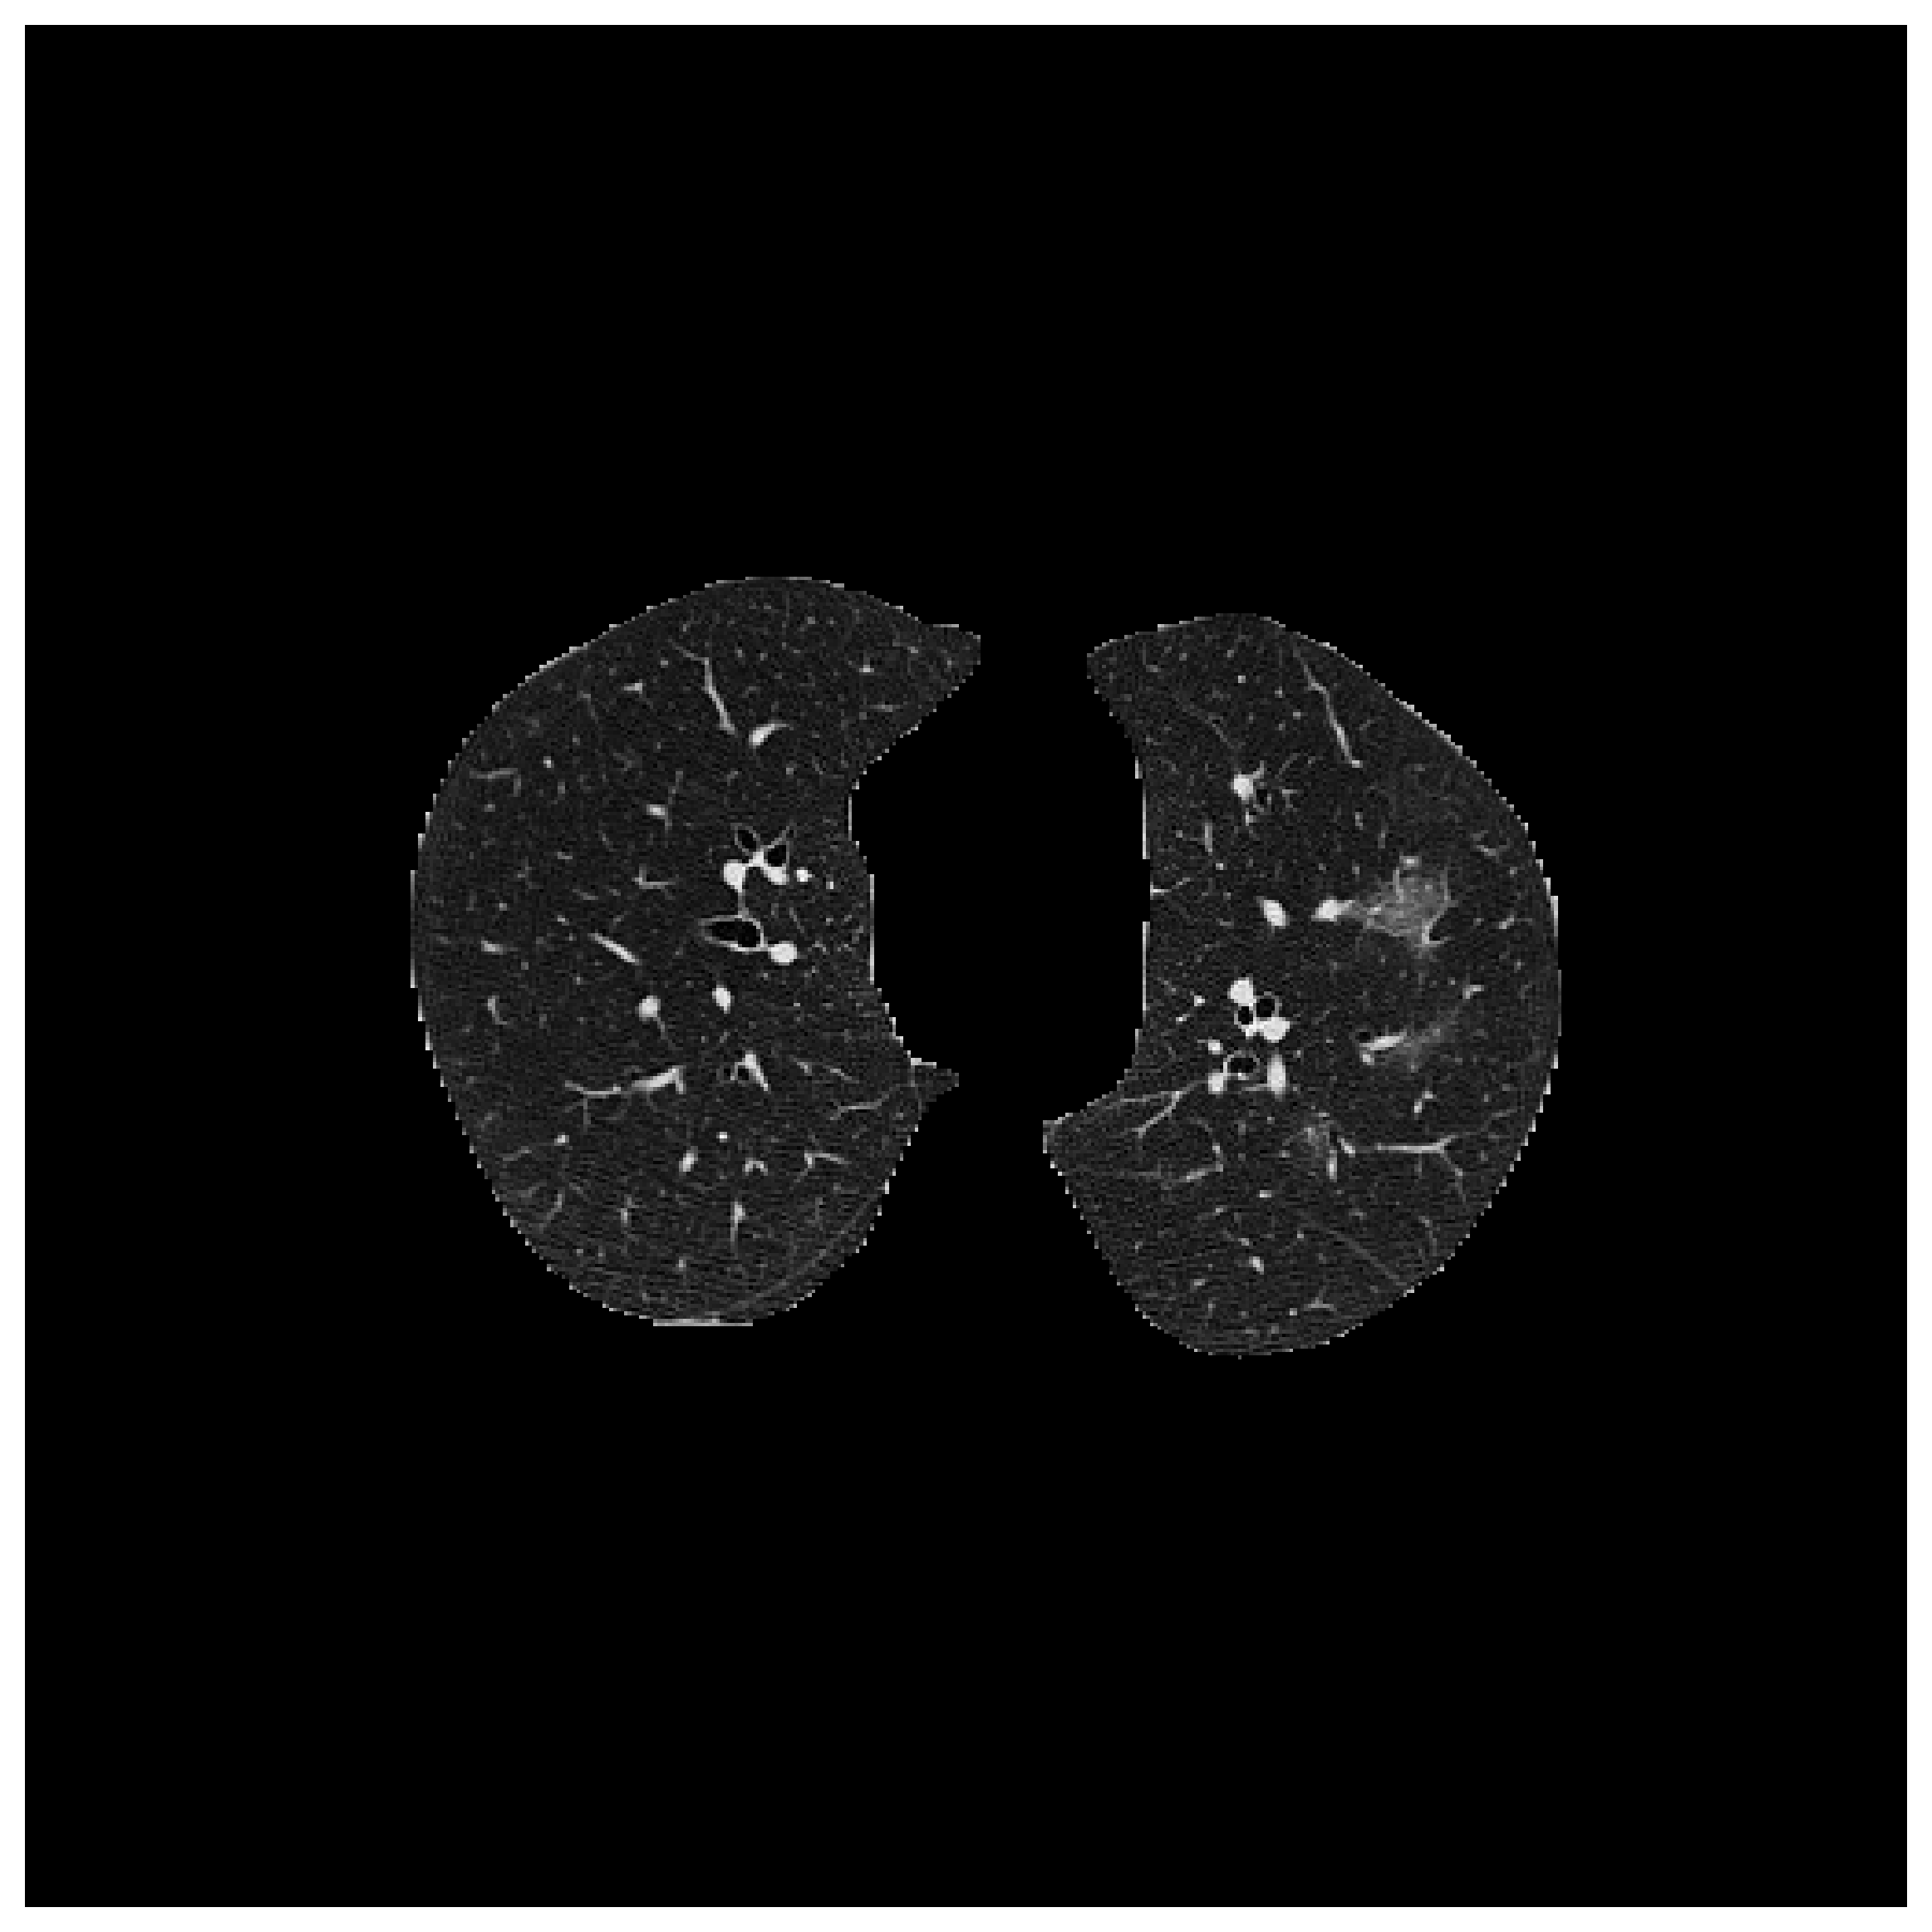
\includegraphics[width=.7\linewidth]{./img/Lung_2}
				\centering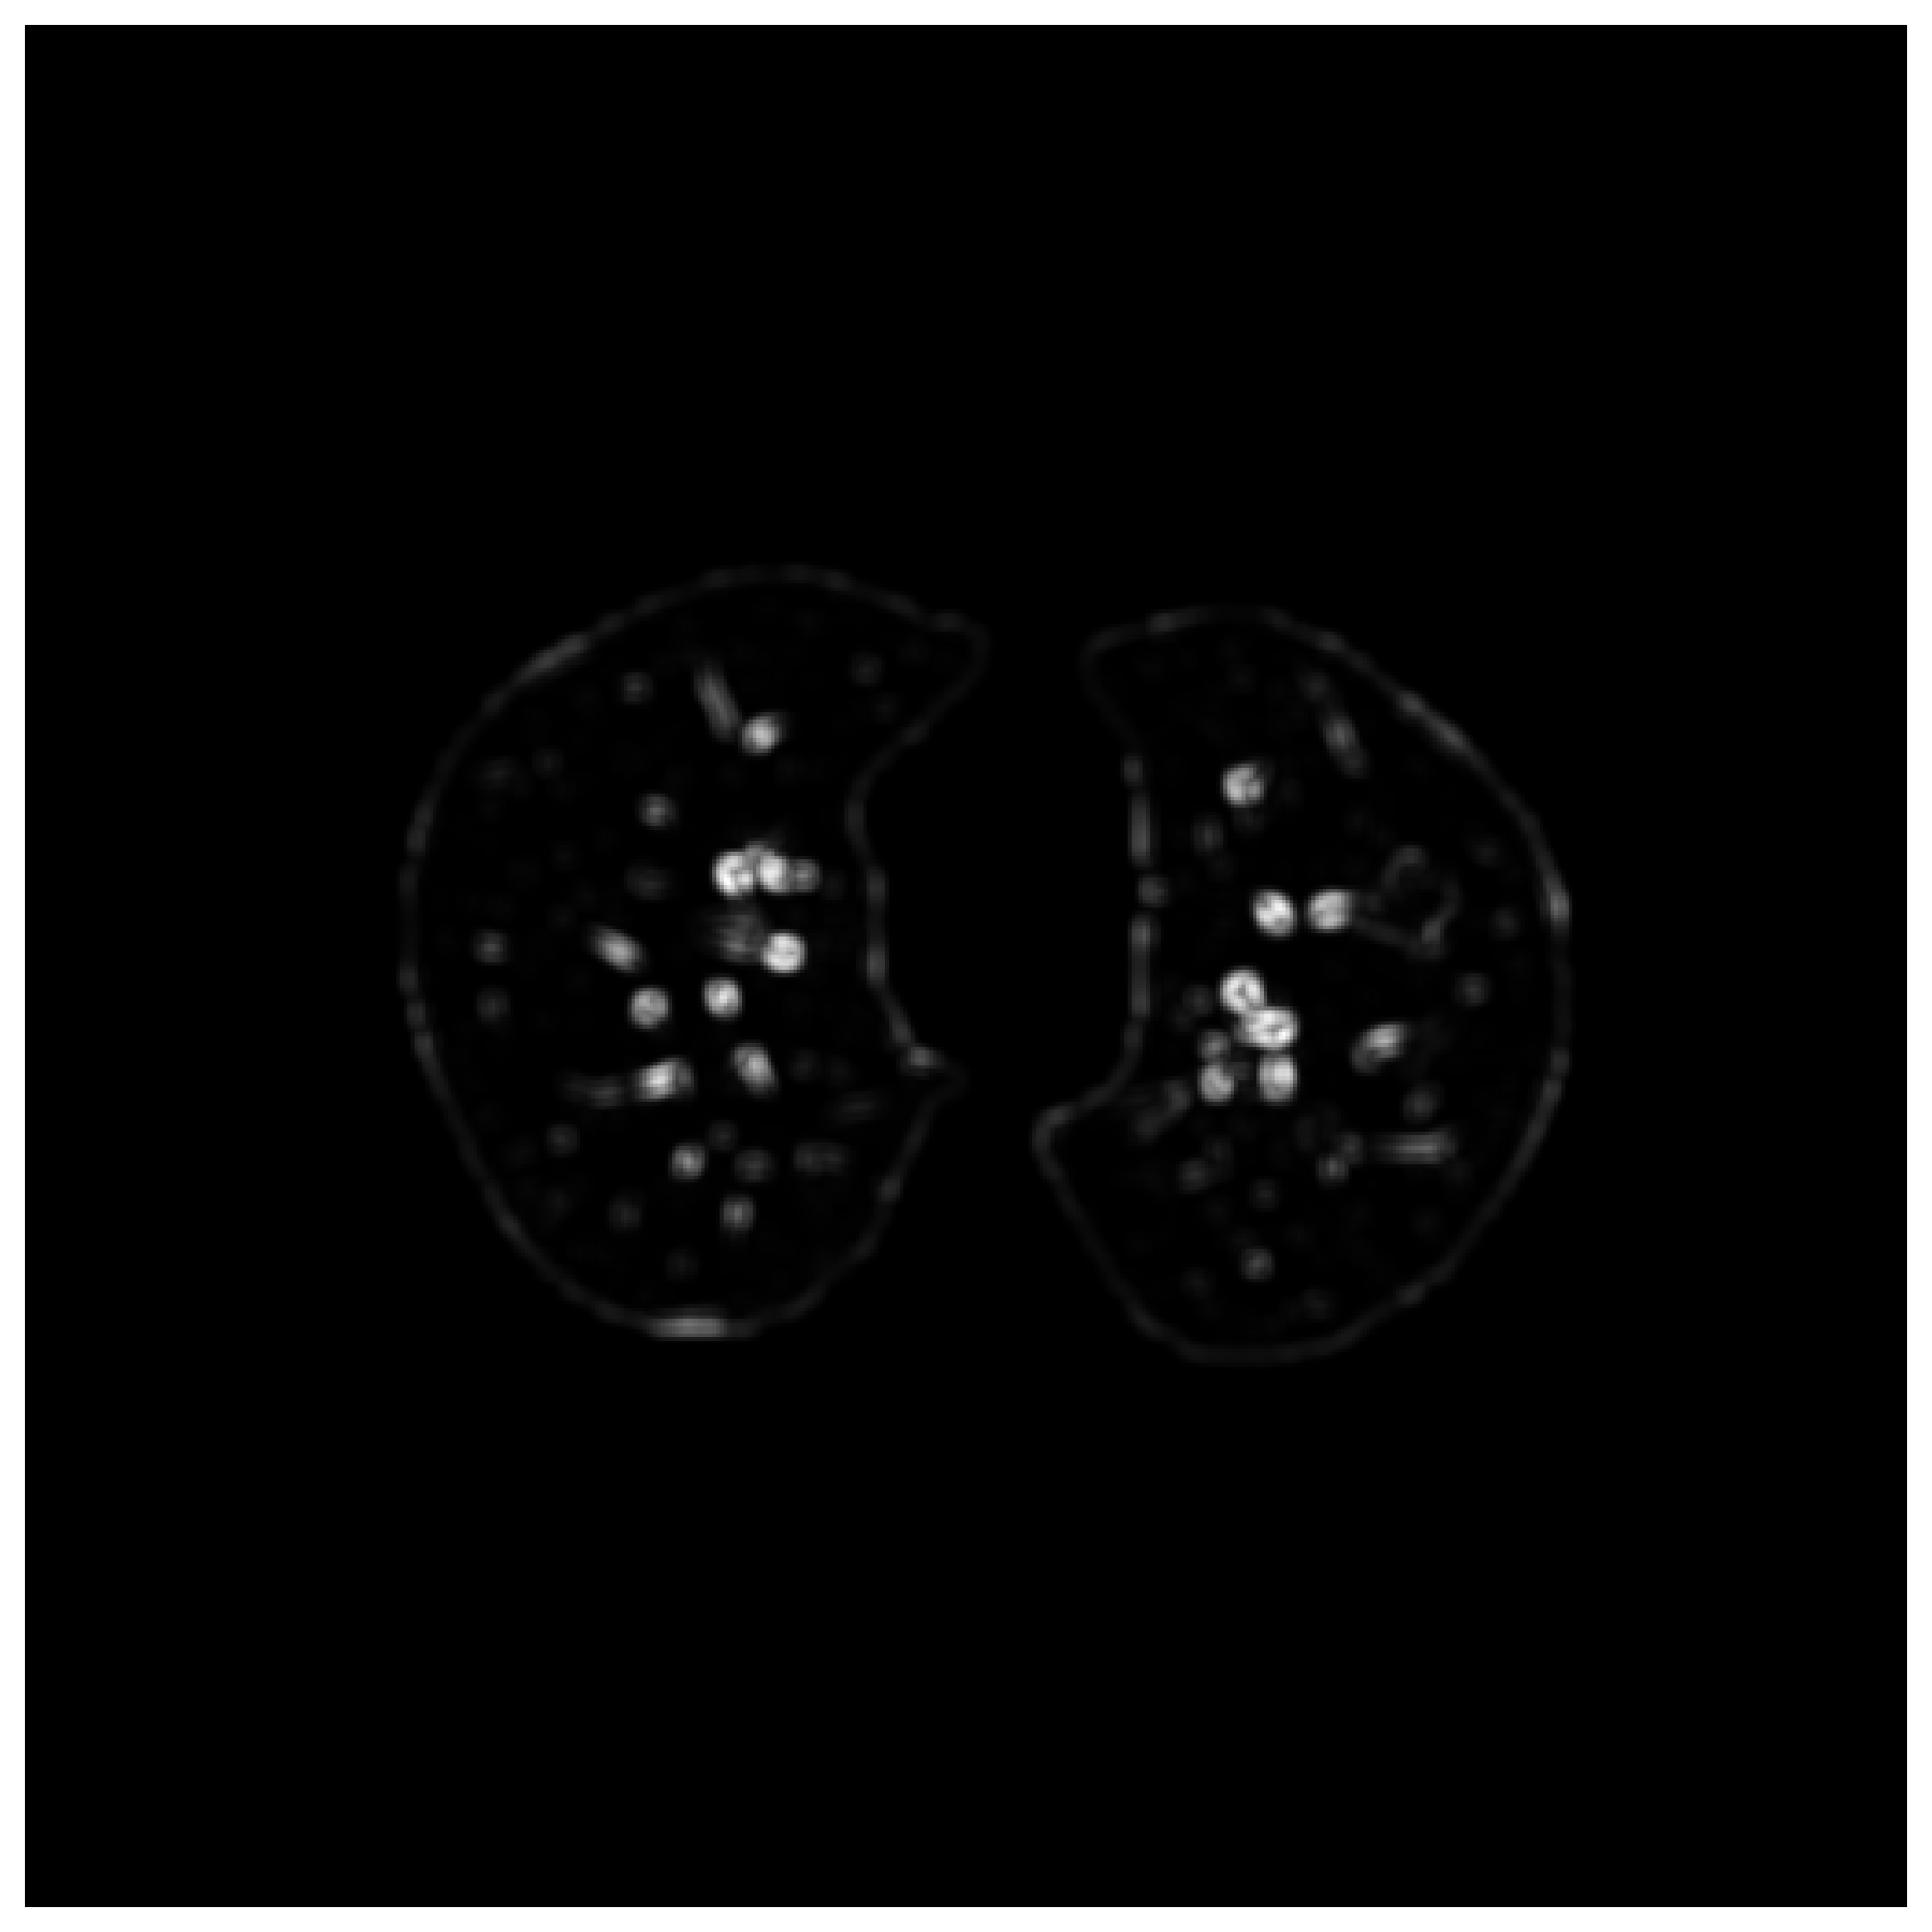
\includegraphics[width=.7\linewidth]{./img/eigmap}
			\end{column}
			\begin{column}{.4\textwidth}
			%\begin{scriptsize}	

				\begin{equation*}
					M = \begin{bmatrix} \sum _{S(p)}(\frac{dI}{dx})^2 & \sum _{S(p)}\frac{dI}{dx}\frac{dI}{dy} \\ \sum _{S(p)}\frac{dI}{dx}\frac{dI}{dx}& \sum _{S(p)}(\frac{dI}{dy})^2 \end{bmatrix}
				\end{equation*}
			%\end{scriptsize}	
		
			\centering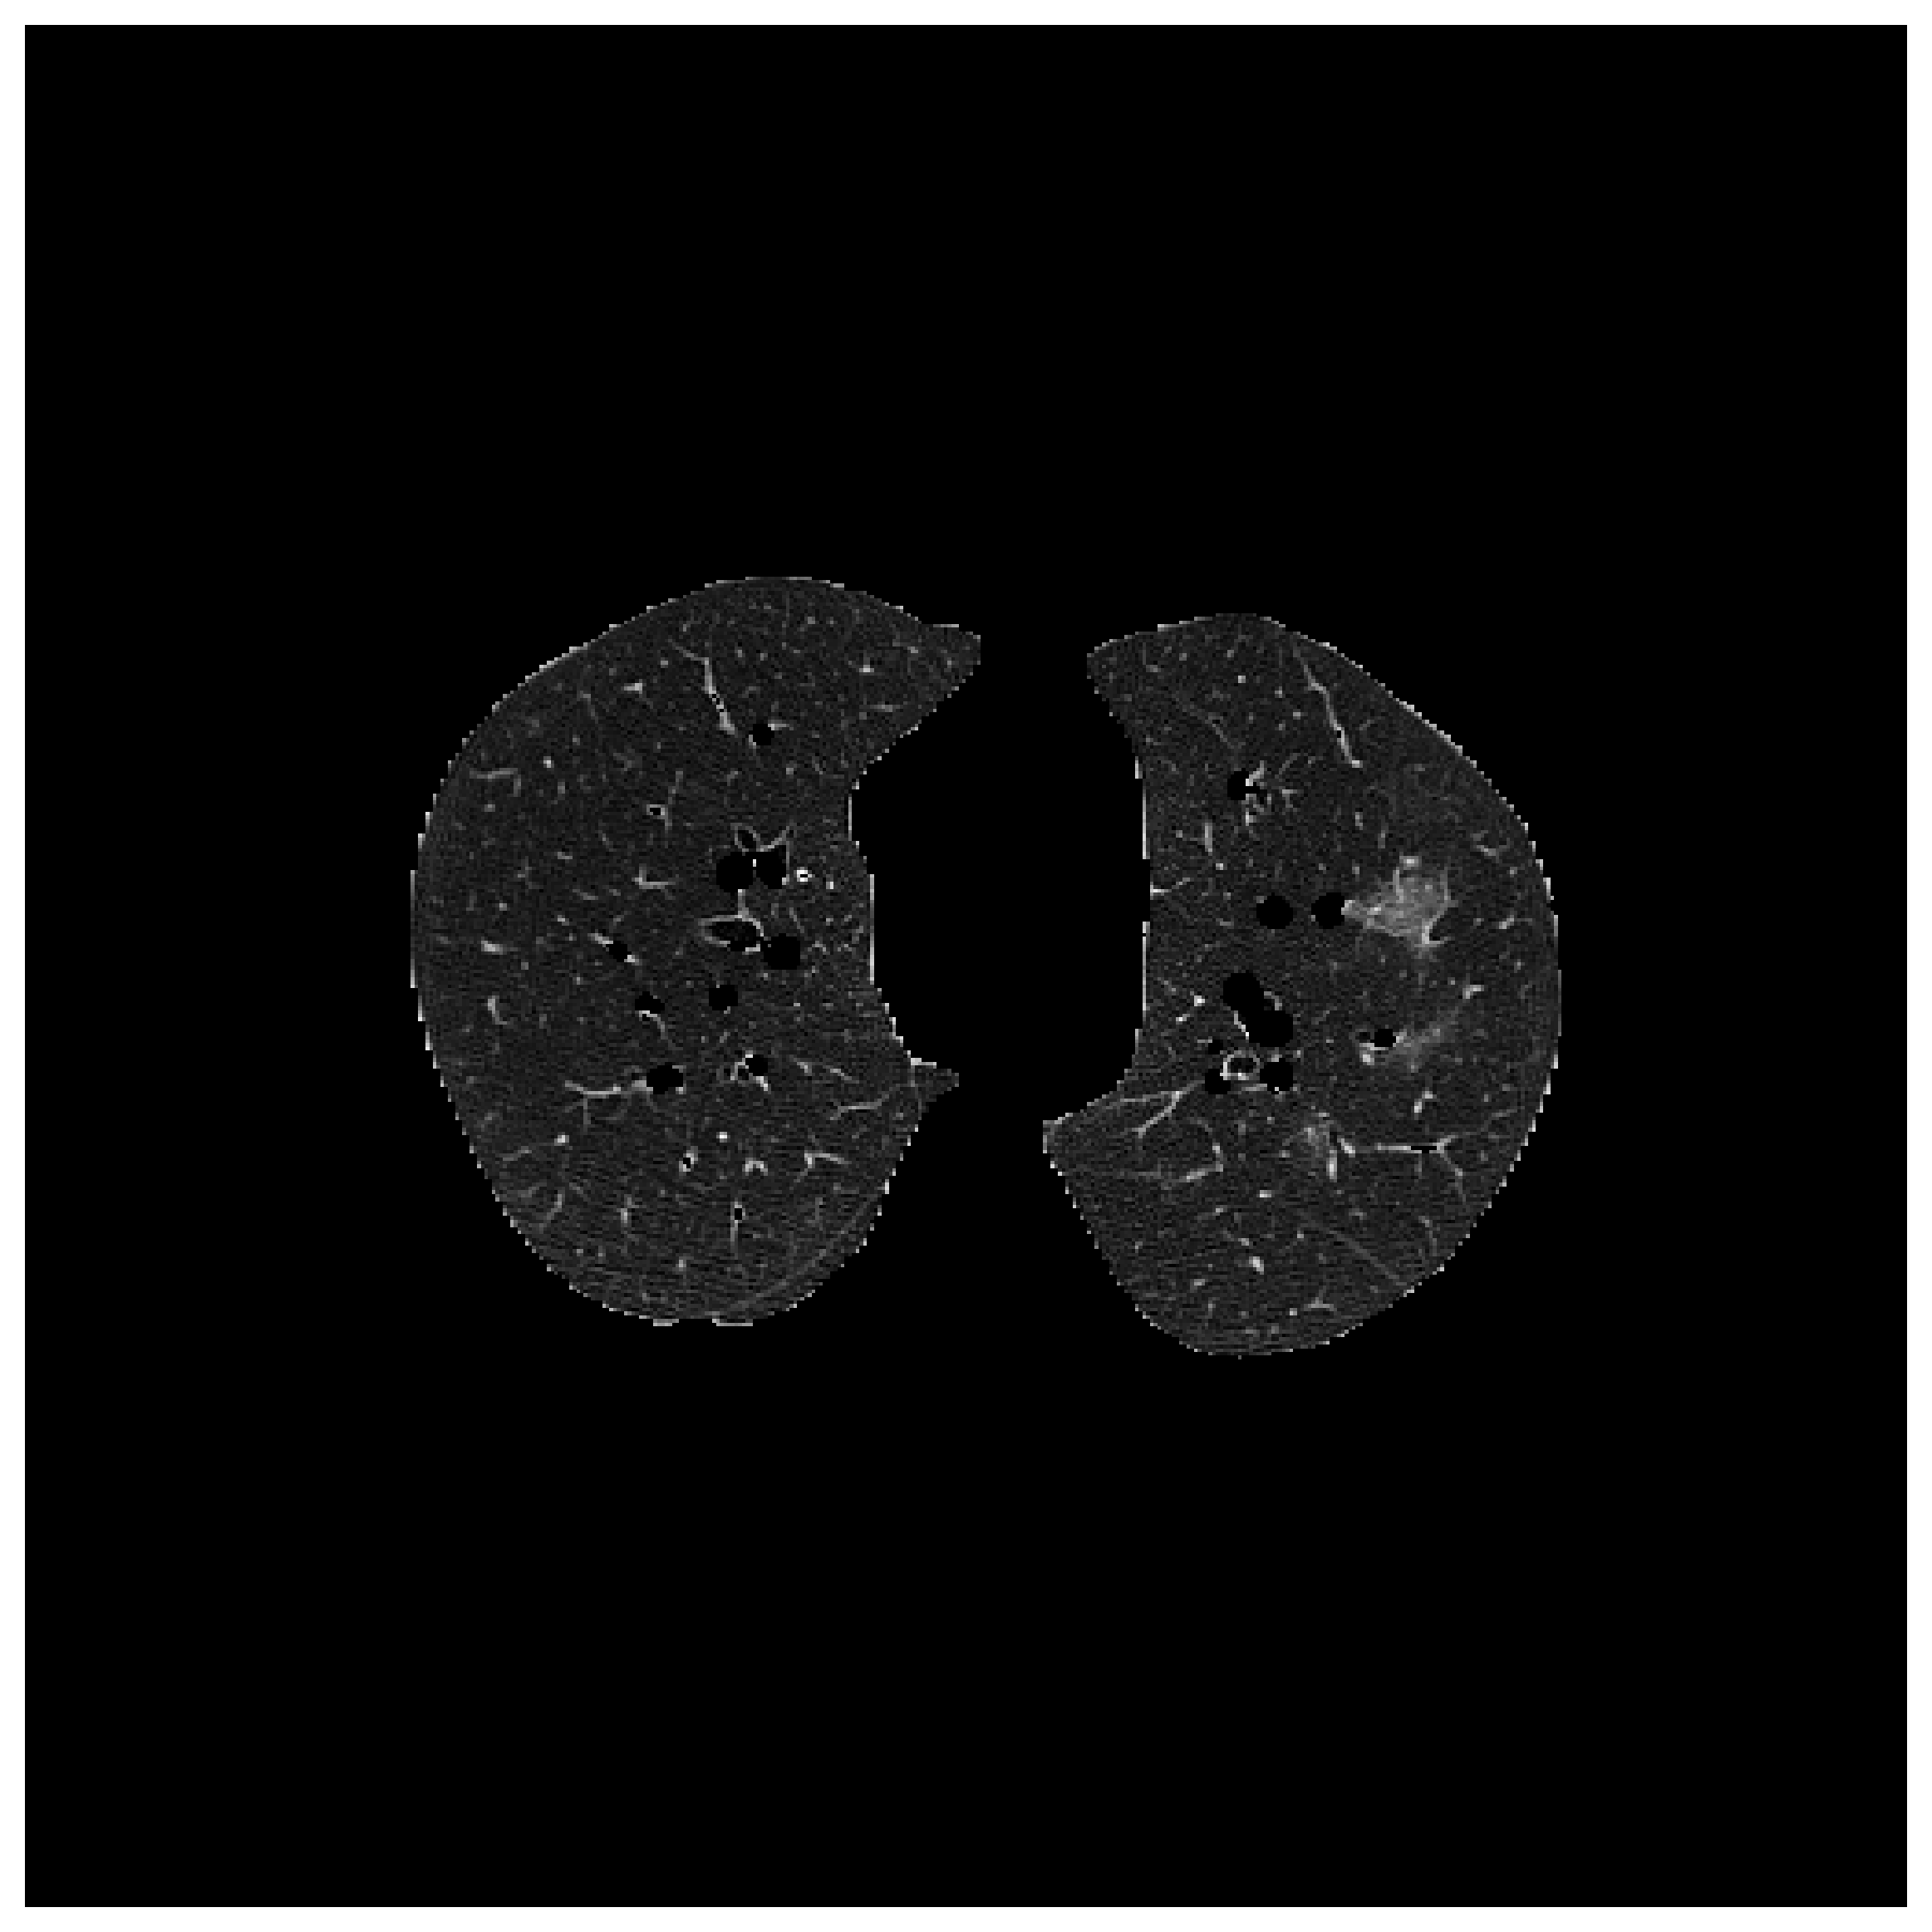
\includegraphics[width=.7\linewidth]{./img/NoBr}
		\end{column}
		\end{columns}
	\end{frame}
\end{document}% Max Eigenvalues Map for bronchial removal

\documentclass{standalone}
\begin{document}
	\begin{frame}[noframenumbering]{Timing}{Measuring the time performances}
		\begin{columns}
			\begin{column}{.6\textwidth}
				\centering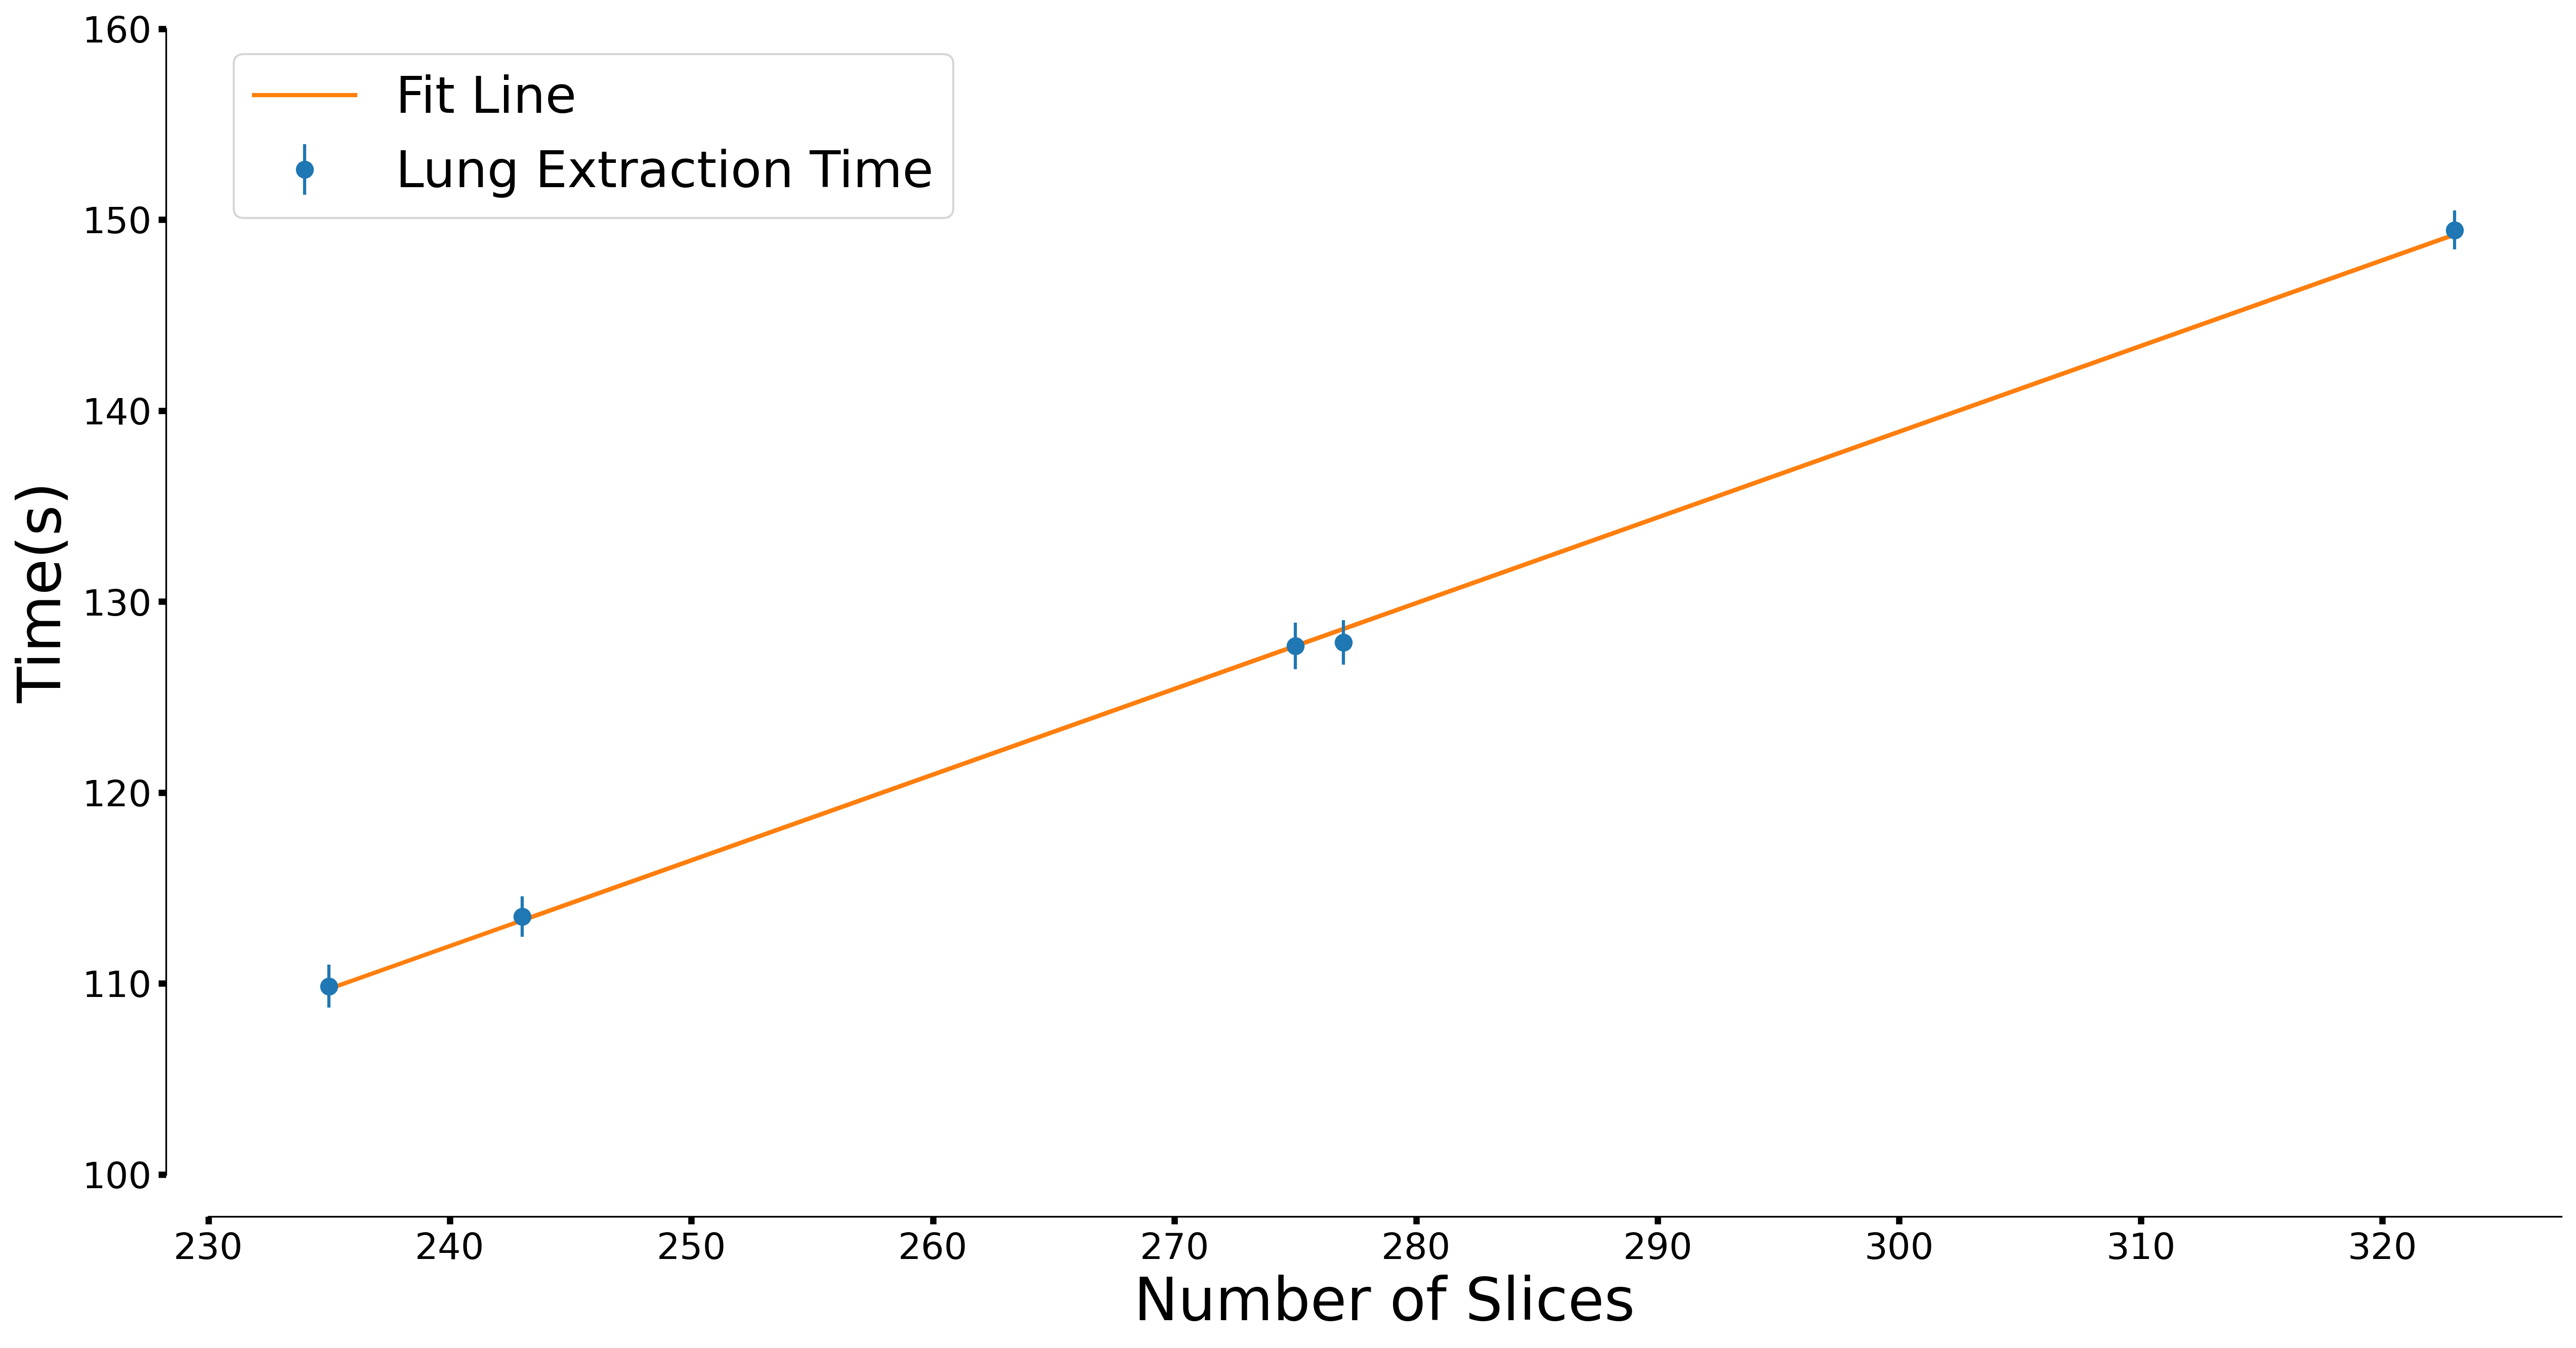
\includegraphics[width=.9\linewidth]{./img/Lung_timing}
				\centering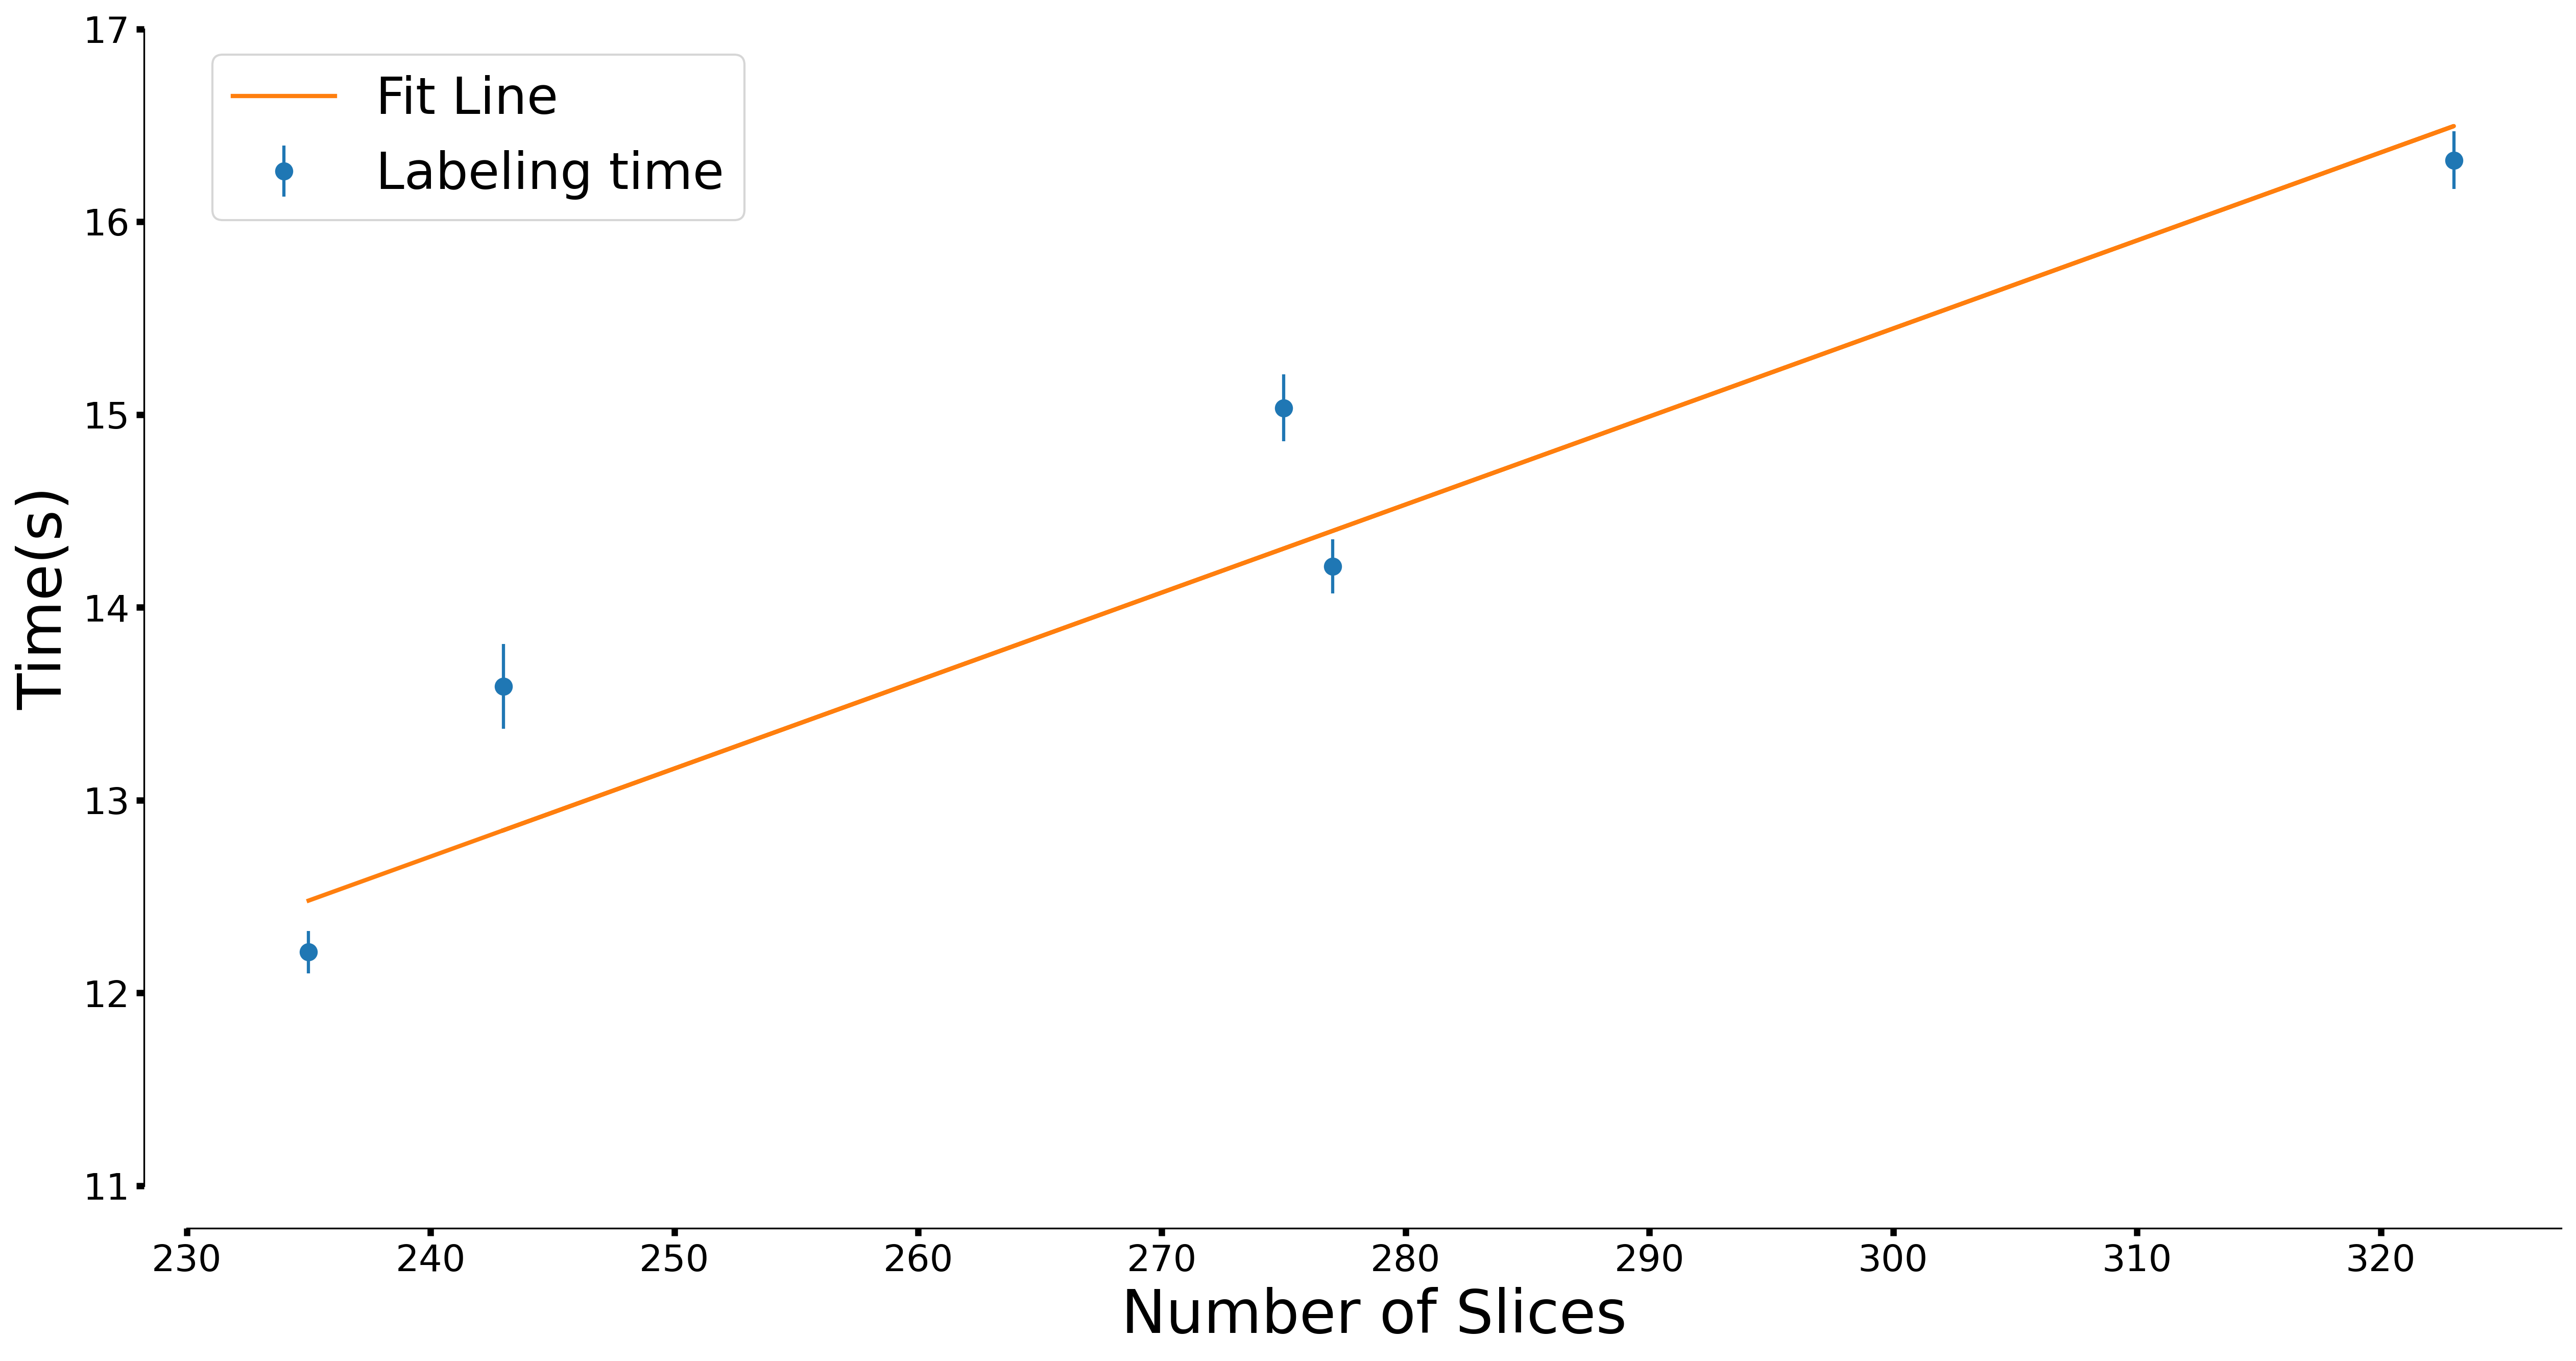
\includegraphics[width=.9\linewidth]{./img/Labels_timing}
			\end{column}
			\begin{column}{.3\textwidth}
				\begin{block}{Time per slice}
					\begin{itemize}
						\item \scriptsize\textbf{Lung Extraction:}$449.94\pm 0.03\,ms$
						\item \scriptsize\textbf{Labelling:}$45.65\pm 0.05\,ms$
					\end{itemize}
				\end{block}
			\end{column}
		\end{columns}
	\end{frame}
\end{document} % How I have measured time performances

\documentclass{standalone}
\begin{document}
	\begin{frame}[noframenumbering]{Results}{Sensitivity and Specificity}
		
		\centering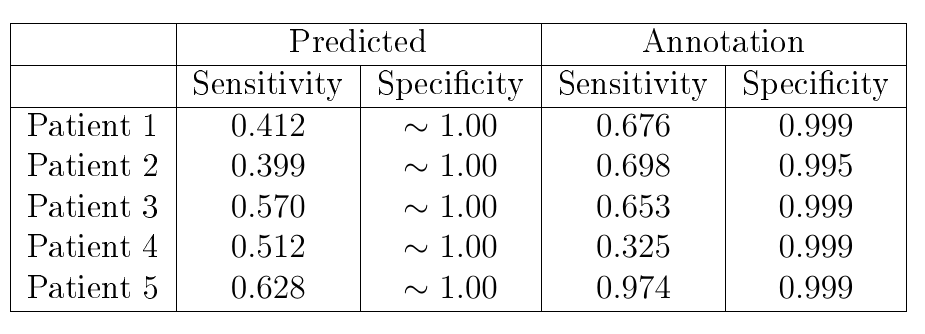
\includegraphics[width=.8\linewidth]{./img/Tabella}
		
		\centering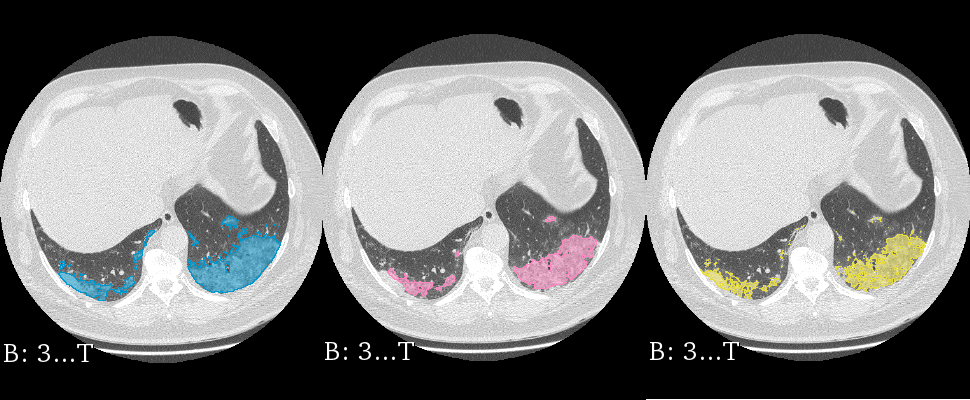
\includegraphics[width=.8\linewidth]{./img/GTCOMP1}
		
	\end{frame}
\end{document} % Specificity and sensitivity

\end{document}